% !TEX encoding = UTF-8 Unicode


% TODO: HIER KIJKEN VOOR STRUCTUUR EN OPMAAK http://tex.stackexchange.com/questions/20538/what-is-the-right-order-when-using-frontmatter-tableofcontents-mainmatter?rq=1



%\documentclass[book,a4paper,12pt,natbib]{apa6}
\documentclass[a4paper,12pt]{book}

\usepackage[titletoc]{appendix}

\newcounter{lijst}

\usepackage[natbibapa,nosectionbib,tocbib,numberedbib]{apacite}



\usepackage[utf8]{inputenc}
\usepackage{graphicx}
%\usepackage{wrapfig}
%\usepackage{xparse}
\usepackage{enumerate}
\usepackage{url}
\usepackage[dvipsnames]{xcolor}
\usepackage[colorinlistoftodos]{todonotes}
\usepackage{hyperref}
\usepackage[scale=2]{ccicons}

%to make line breaks possible at more parts within \texttt
\renewcommand{\texttt}[1]{%
  \begingroup
  \ttfamily
  \begingroup\lccode`~=`/\lowercase{\endgroup\def~}{/\discretionary{}{}{}}%
  \begingroup\lccode`~=`[\lowercase{\endgroup\def~}{[\discretionary{}{}{}}%
  \begingroup\lccode`~=`.\lowercase{\endgroup\def~}{.\discretionary{}{}{}}%
  \begingroup\lccode`~=`(\lowercase{\endgroup\def~}{(\discretionary{}{}{}}%
  \catcode`/=\active\catcode`[=\active\catcode`.=\active\catcode`(=\active
  \scantokens{#1\noexpand}%
  \endgroup
}



\usepackage{lettrine}

\usepackage{lmodern}
\usepackage{listings}
\lstset{
basicstyle=\footnotesize\ttfamily,
columns=flexible,
breaklines=true,
numbers=left,
%stepsize=1,
numberstyle=\tiny,
backgroundcolor=\color[rgb]{0.85,0.90,1}
}


\lstnewenvironment{lstlistingbash}{\lstset{basicstyle=\footnotesize\ttfamily,
		columns=flexible,
		breaklines=true,
		numbers=left,
		%stepsize=1,
		numberstyle=\tiny,
		backgroundcolor=\color[rgb]{1,0,.4}}}{}


\lstnewenvironment{lstlistingoutput}{\lstset{basicstyle=\footnotesize\ttfamily,
		columns=flexible,
		breaklines=true,
		numbers=left,
		%stepsize=1,
		numberstyle=\tiny,
		backgroundcolor=\color[rgb]{.7,.7,.7}}}{}


%\let\oldquote\quote
%\let\endoldquote\endquote

%\RenewDocumentEnvironment{quote}{m}{
%    \oldquote\small\begin{wrapfigure}{l}{2cm}\centering\includegraphics[width=1cm]{gloeilamp.jpg}%
%	\end{wrapfigure}}
%{
%    \endoldquote
%}



\let\oldquote\quote
\let\endoldquote\endquote
\renewenvironment{quote}{
%{
%\setlength{\columnsep}{0pt}%
%\begin{wrapfigure}{l!}[-2cm]{1cm}\vspace*{\topsep}\includegraphics[width=1cm]{gloeilamp.jpg}\end%{wrapfigure}
%}
\oldquote\footnotesize
\lettrine[lines=3]{\color{BrickRed}!}{ }}
{\endoldquote}



\newenvironment{question}{
%{
%\setlength{\columnsep}{0pt}%
%\begin{wrapfigure}{l!}[-2cm]{1cm}\vspace*{\topsep}\includegraphics[width=1cm]{gloeilamp.jpg}\end%{wrapfigure}
%}
\oldquote\footnotesize
\lettrine[lines=3]{\color{BrickRed}?}{ }}
{\endoldquote}


%\title{Big Data and Automated Content Analysis}
\title{Doing Computational Social Science with Python: An Introduction}
\author{Damian Trilling}
\date{Version 0.99\\ ~ \\  \footnotesize{PDF created \today}}


\begin{document}

\frontmatter

\maketitle

\newpage

{~\vfill
\thispagestyle{empty}
\setlength{\parindent}{0pt}
\setlength{\parskip}{\baselineskip}
Copyright \copyright\ \the\year\ Damian Trilling\\
\vspace{.25cm} \\
This document can be obtained from \url{http://papers.ssrn.com/abstract=2737682}. The source code of the most recent version can be found at \url{https://github.com/damian0604/bdaca}.


\par Licensed under the Creative Commons Attribution-NonCommercial-NoDerivatives 4.0 International License. You may obtain a copy of the license at \url{http://creativecommons.org/licenses/ by-nc-nd/4.0/}. \\
\vspace{.5cm} \\
\ccbyncnd

}


\newpage

\tableofcontents


\chapter{Introduction: What and why?}

Social scientists are more and more confronted with the analysis of large-scale datasets. Often, these are data from online sources, and often, they contain some form of textual data. Think of data from social media, but also large archives. Often, this development if referred to as a move towards ``computational social science'' \citep{Lazer2009,Kitchin2014}.

There is a certain overlap with the term ``Big Data''. But although the latter sounds sexy, it is a somewhat problematic term, because people use it for all kind of data. As scientists, we want a clear definition, but it is hard to tell what the term Big Data actually entails. This document is not about \emph{really} Big Data requiring a whole server farm, but it is about data that is too big to handle manually---think of one million tweets for example. It is about data sets that are small enough to be handled by an ordinary desktop computer, but often too big to be processed by ordinary programs. Excel does not have an unlimited number of rows, and SPSS and STATA start complaining (or simply stop working) once you have too many cases and variables. If you know R, you are better off, but for some of the tasks we will discuss in this document, Python has a bit more to offer.\footnote{I do not want to go into the R-vs-Python-for-data-analysis debate here, I use both tools, but for different tasks. Google for it if you want some comparison.}  

This document introduces you to automated content analysis of data that typically comes in amounts that are too voluminous for manual coding and for traditional point-and-click applications: Tweets, blogposts, articles from RSS-feeds, etc. We will use the programming language Python, which is very flexible and highly suitable for this end. It also scales very nicely---meaning that you can use it now for some smaller projects, but it can also be used on immense data sets. So, if you will find yourself working on some really Big Data that cannot be handled on a single computer any more, the principles are not too different from what we do in this document (yes, I'm simplifying a bit).

You will be guided through the first steps towards automated content analysis with Python. Note that I wrote this document for an audience of students in the social sciences, communication science in particular. From a computer science point of view, much more would have to be said, and some things we do in this course might actually be considered bad programming style. But that's not our objective here: This course should enable students of the social science to make some first steps with Python, in order to solve their analytical questions.

This also means that this manual is far from complete. It rather serves as a starting point---and from that point onwards, it's up to you. Once you got the basic ideas and concepts, there are enough resources out there to help you further.

Have fun! And, join me in thanking those who contributed with great ideas or served as guinea pig for earlier versions of this document -- which basically applies to all students and colleagues working with earlier versions of this document. 

\vspace{.5cm}

\begin{flushright}
Amsterdam, March 2015 (version 0.1)\\
Amsterdam, February 2016 (version 0.2)\\
Amsterdam, January 2017 (version 1.0)
\end{flushright}

Damian



\begin{flushright}
~\\~\\Damian Trilling\\
d.c.trilling@uva.nl\\
www.damiantrilling.net\\
@damian0604

\end{flushright}

\chapter{How to read this book}
\label{howtoread}

Before we start, let me introduce three conventions that I'll use in this book. Python-code, which you will type into the Python interpreter or use in the programs you'll write, is represented in blue:
\begin{lstlisting}
print("Hello world"!)
\end{lstlisting}
Commands that you have to type into the Linux command line (also referred to as shell, terminal, or bash) are pink:
\begin{lstlistingbash}
echo Hello world!
\end{lstlistingbash}
And any output or data file is represented in gray:
\begin{lstlistingoutput}
Hello world!
\end{lstlistingoutput}

And a word about the structure of this book. Part \ref{part:basics} teaches you the basics and should be read in the structure as presented in the book, as the chapters build on each other. 

Part \ref{part:specific} presents specific techniques and can be read in any order you like. While there are some cross-references between the chapters, they do not necessarily build on each other. However, it assumes that you have all knowledge from Part \ref{part:basics}, and, most importantly, that you installed everything as explained in Chapter~\ref{chap:prepare}.

Nevertheless, there are two ways to work with this book: the complete route and the short route.

\section*{The complete route}
When you use this book as part of a multi-week course, this is the route you take: You start at the beginning of and end, well, at the end (maybe skipping a bit here and there, or using some extra materials in addition.)

\section*{The short route}
When you use this book as a part of a short one or two day course, then you probably do not have the time to work through all materials. If the course focuses on just a few chapters from Part~\ref{part:specific}, the following preparations might be sufficient (if you do not want to fully read through Part~\ref{part:basics}):
\begin{itemize}
\item Make sure you have a basic understanding of the Python language, for example by following an online course like this one: \url{https://www.codecademy.com/learn/python}
	\item Install Anaconda (the version for Python 3, not 2) from  \url{https://www.continuum.io/downloads}. Anaconda is a Python distribution that already includes most packages that you might want to use (see also Appendix~\ref{chap:anaconda}). Most likely, you will work using Jupyter Notebooks (Section~\ref{sec:jupyter}), so make sure you know how to start it!
\end{itemize}
Please note that when you use the short route, you will not be able to follow all instructions and examples in this book by the letter, especially because some of them imply that you are working on a Linux system (which you were, if you followed the approach of the long route, but probably aren't otherwise).



\mainmatter

\part{Basics}
\label{part:basics}

\chapter{Preparing your computer}
\label{chap:prepare}

This chapter describes how to prepare your computer. We work with so-called virtual machines, which means that we install a program within which you can install an own operating system. This means that
\begin{enumerate}[(a)] 
\item you can play around without the danger of damaging your own system;
\item you can make use of a lot of cool tools that might not be available for your own system;
\item everyone in this course has exactly the same environment running.
\end{enumerate}

Specifically, we are using Oracle VirtualBox, within which we will install Lubuntu (a lightweight version of Ubuntu, a user-friendly Linux distribution). Before you start, make sure that you have plenty of space available on your laptop, preferably more than 10 GB. (You'd better put your music and photos on an external drive for the duration of this course...)

\textbf{Before you continue, make sure you have read ``How to read this book'' on page~\pageref{howtoread}.}

Ready to go?



\section{Install VirtualBox}
Download and install VirtualBox from \url{https://www.virtualbox.org/}. Depending on your computer, download the binary for Windows, MacOS, or Linux.

\section{Download a Lubuntu-image}
Download the Lubuntu image from \url{http://lubuntu.net}. \textbf{We are working with version 16.04.1 LTS (Xenial Xerus). It is important that you do \emph{not} use version 16.10.} The download link for this version should be \url{http://cdimages.ubuntu.com/lubuntu/releases/xenial/release/}
If you have a reasonably new computer, download \texttt{lubuntu 64-bit (AMD64) desktop CD}, only if you encounter problems later on or have an old computer (up to around 2007), download the 32-bit version. So, in most cases, select the 64-bit Desktop version (\texttt{lubuntu-16.04.1-desktop-amd64.iso}). 
Save it at a place of your convenience.

\section{Create a virtual machine}
Open VirtualBox, click on ``New'', give your image a name, and select first Linux, then Ubuntu~64bit from the list (or 32 bit, if that's what you downloaded). On the following screens, just leave the default settings and agree to everything---with one exception: When you are asked how much ``base memory'' you want to allocate to your machine, you should choose a value of at the \emph{very} least around 1000 MB. More is better, if you you have 4,096 MB of RAM in total, you can safely choose 2,048 MB. The examples in this tutorial are tested on a VM with 2,048 MB RAM. 

On the next screens, you are asked about a virtual hard disk to create. I strongly recommend you to use a bit more than the 8~GB that are suggested. If you choose more (say, 12~GB or so), chances are lower that you will run out of space later during the course.

\begin{quote}
The virtual machine you just created should show up in the main window now. If it doesn't (I had that on one computer once), restart VirtualBox.
\end{quote}


\begin{figure}[h]
	\centering
	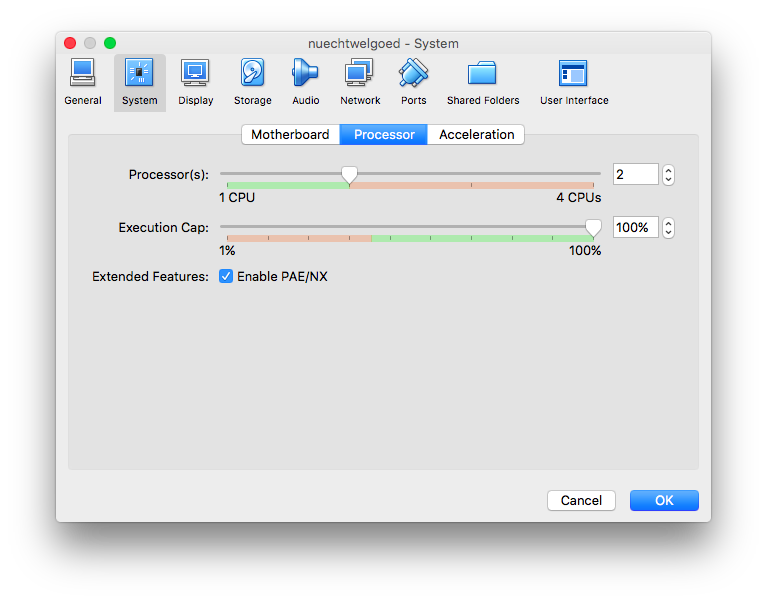
\includegraphics[width=.5\paperwidth,,keepaspectratio]{../pictures/virtualbox-tweak2.png}
	\caption{\label{fig:tweak2}Possibly necessary tweaks: Enabling PAE/NX and allowing the use of multiple CPUs in the settings dialogue}
\end{figure}


\begin{figure}[h]
\centering
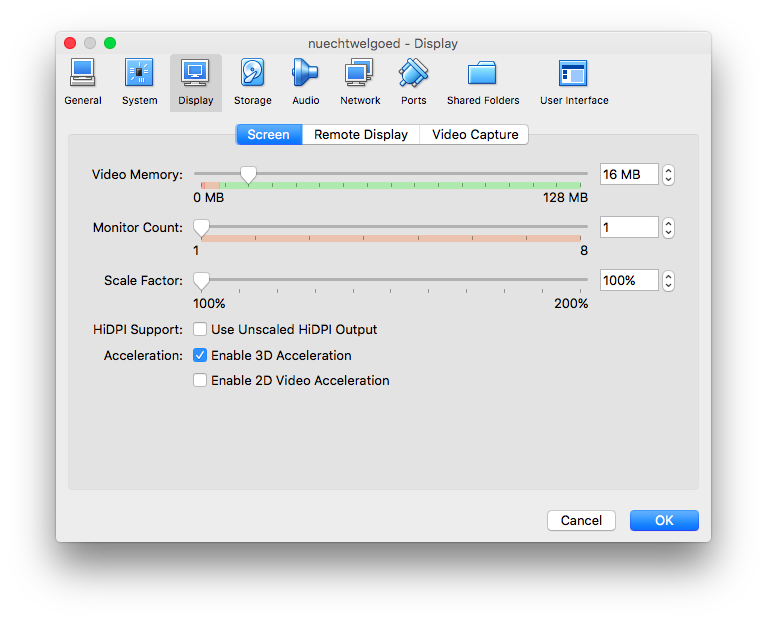
\includegraphics[width=.5\paperwidth,,keepaspectratio]{../pictures/virtualbox-tweak1.png}
\caption{\label{fig:tweak1}Possibly necessary tweaks: Enabling 3D and/or 2D acceleration in the settings dialogue}
\end{figure}



Now click on the name of the virtual machine and on "Settings" (Figure~\ref{fig:tweak2}. Under "System"/"Processors", you should see a check box "Enable PAE/NX". If you can enable this, enable it.\footnote{In rare cases, you might just to have to disable it. So, if you cannot start your VM, you know what to try.} If you have more than one processor, also select the maximum (e.g., choose 2 instead of 1). Confirm with OK. Also, check if you can enable "Display"/"Enable 3D acceleation" (Figure~\ref{fig:tweak1}). These changes might not be strictly necessary, but can in some instances prevent problems.

When you are done, start the virtual machine by clicking on the green arrow in the main window. You will be asked for a location from which to boot. Click on the icon to select a file and select the Lubuntu-image you downloaded.


\section{Install Lubuntu on your virtual machine}
Once your virtual machine is running, you can select whether you want to try out Lubuntu without installing or install it. If you feel like, you can now just play around a bit in the try-out mode, but eventually, you'll need to go for installing as we need some specific tools for our course. So you can as well just select Install now, using the arrow keys.
When you select "Install", just follow the instructions. At one point in time, you will be asked whether you want to erase all data from your hard drive (yes, seriously). You can safely agree (remember, that's just the point of the VirtualBox, you have a fenced room in which you cannot damage anything. Only your \emph{virtual} hard drive will be erased, not your real one).
After finishing the installation, your virtual machine will reboot. After clicking on reboot, you can get a message saying ``please remove installation disks''. You can just press enter, you don't have to remove anything in your case. Also, it might happen that you see only some lines of text saying something like ``Unmounting crypto disks''. If this takes longer than a minute or so, try pressing Enter twice. 



\section{Install necessary packages}
\label{sec:installpackages}
Once you have installed and rebooted your virtual machine, you will have to install a couple of packages. It might be that your system is running now in a very low resulution, but that will change after the following step.  Click on the button on the bottom left (where the traditional Windows start button would be), then on System Tools/LXTerminal. Enter the following command:
\begin{lstlistingbash}
sudo apt-get install virtualbox-guest-dkms virtualbox-guest-utils virtualbox-guest-x11
\end{lstlistingbash}
You will be asked for your password (the one you defined during the install process). Just type it and confirm with Enter (no, you do not see anything while you type, that's correct). 
If you reboot your virtual machine (by clicking on the Start button/logout/reboot or by typing
\begin{lstlistingbash}
sudo reboot
\end{lstlistingbash}
it will display in a higher resolution and you can even run it full screen if you want to (by clicking on View/Switch to Full Screen in the VirtualBox menu).

We will now install some other programs we will use with the following commands. Just type them into the LX Terminal, which you already know:

\begin{lstlistingbash}
sudo apt-get install gedit spyder3 python3-dev python3-pip
\end{lstlistingbash}

You will be asked for your password and some questions which have to be answered with yes (by typing the letter \texttt{y}) followed by Enter. 

Let us also update everything to the latest version:

\begin{lstlistingbash}
sudo apt-get update
sudo apt-get upgrade
\end{lstlistingbash}


And let us finally install some additional Python modules:

% als we apt-get install python3-pip doen, dan krijgen we een verouderde versie van pi wat later tot problemen leidt

\begin{lstlistingbash}
sudo pip3 install --upgrade pip
sudo pip3 install nltk
sudo pip3 install scikit-learn
sudo pip3 install pandas
sudo pip3 install statsmodels
sudo pip3 install jupyter
sudo pip3 install gensim
\end{lstlistingbash}

In the start menu under "Education" you now find a new program, Spyder~3. This is the tool we will be using for doing some Python programming. But of course, you can also start it from the command line by just typing:

\begin{lstlistingbash}
spyder3 &
\end{lstlistingbash}


\begin{quote}
	While working in the VM, you realize that you made a mistake while configuring your keyboard so that some keys don't work as expected? No worries, you can re-configure your keyboard at any time with the following command:\\
	\texttt{sudo dpkg-reconfigure keyboard-configuration}\\
	If you have a standard laptop purchased in the Netherlands, it is very likely that you have a US keyboard. In that case, the following configuration is correct:\\ 
	Model: Algemeen 105 toetsen internationaal\\
	Oorsprong van het toetsenbord (Engels VS)\\
	Indeling: Engels (VS)\\
	standaard\\
	geen samenstelling\\
	X-server: nee	
\end{quote}


\section{Recap}
Make sure you installed \emph{everything} correctly. If you got any error messages, try to find out what went wrong or ask your instructor. In particular, make sure you write down \emph{what} went wrong.

There are so many different system types (and believe me, I never expected \emph{how} many slightly different systems there are until I had dozens of students in these methods courses!), that we cannot cover every eventuality. But once you got your VM is up and running, everything should be the same for everyone in the course.



\chapter{The Linux command line}
\label{chap:commandline}
\section{Getting to know it}
This chapter provides you with some basic knowledge about how to use the command line of your operating system.  Chances are very high that you will need this later, so before diving into Python, I recommend doing this first.
\begin{figure}[h]
\centering
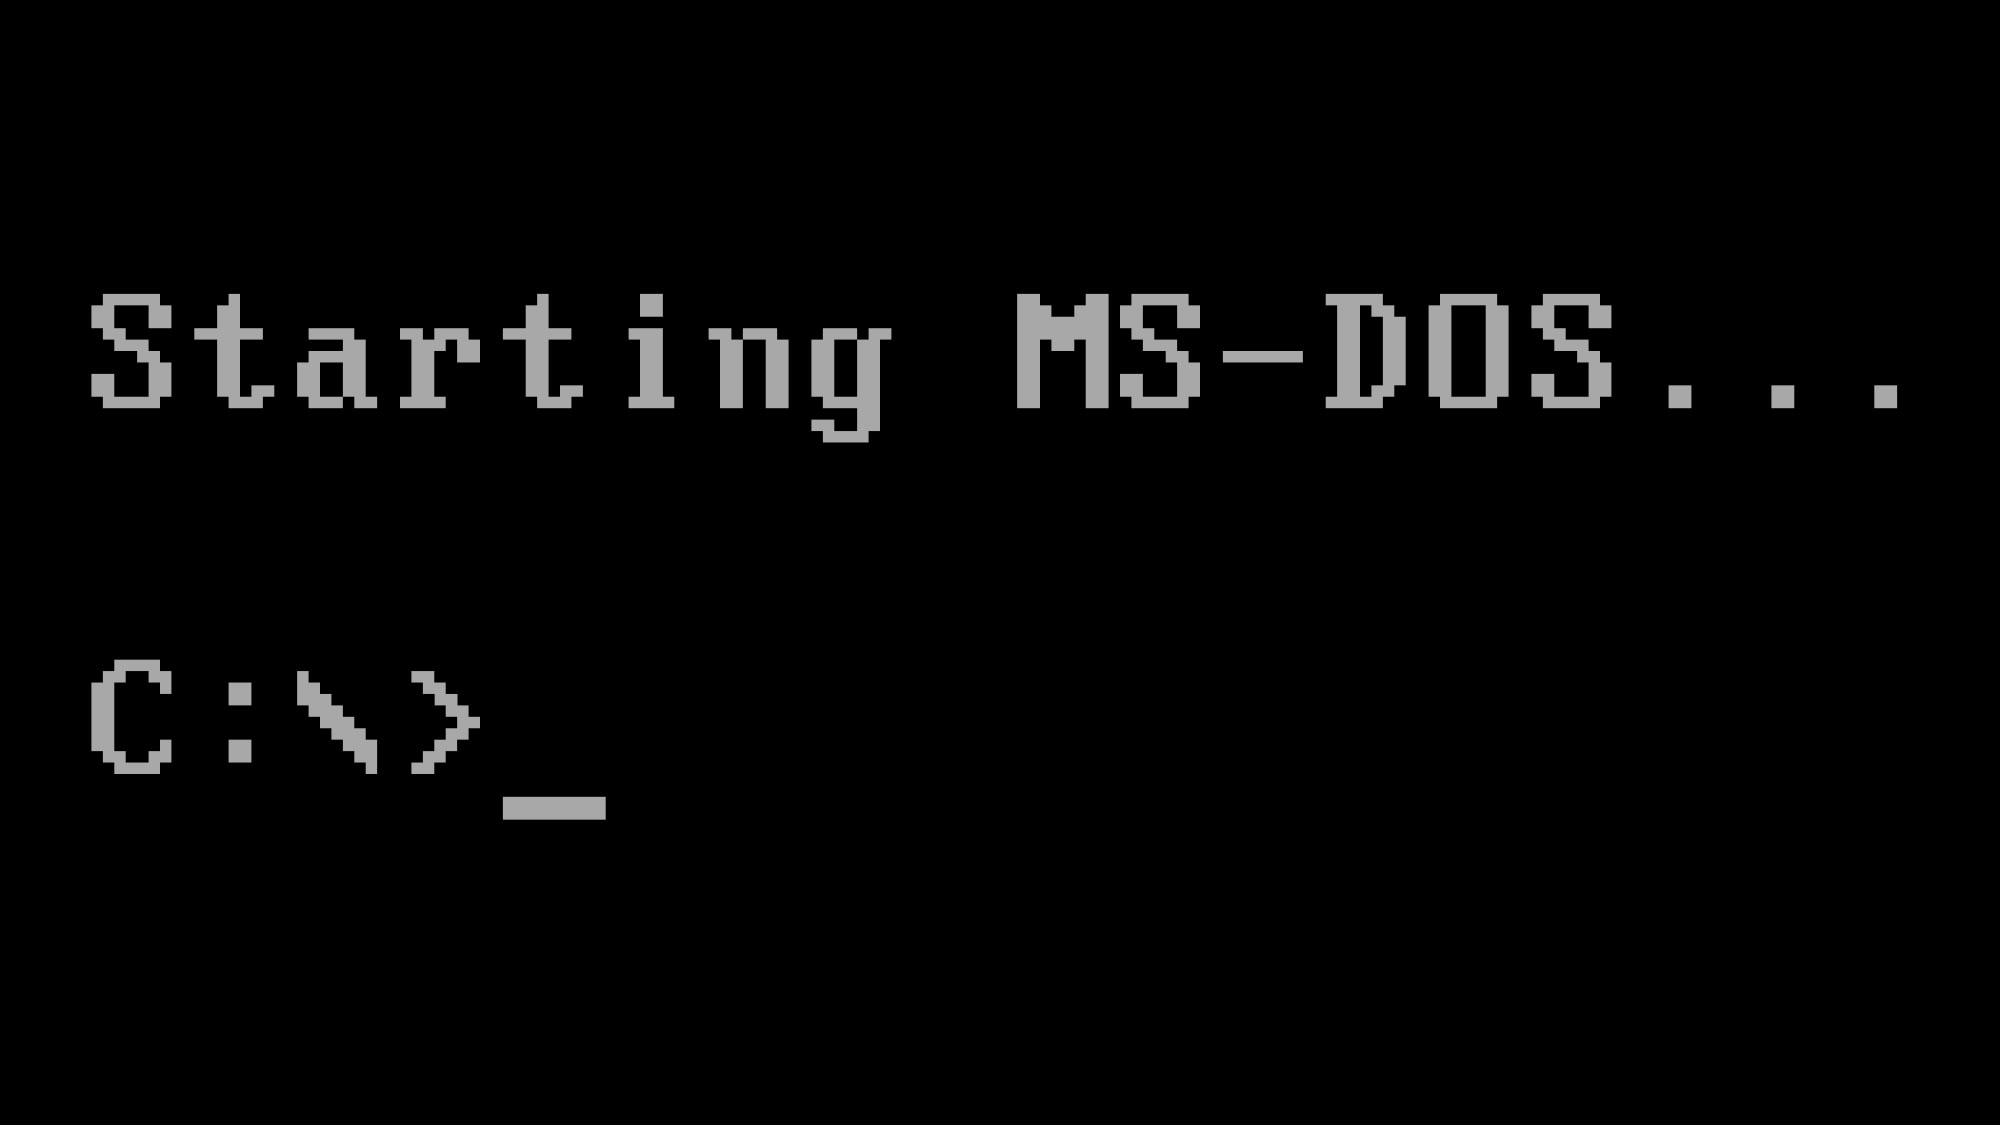
\includegraphics[width=.3\paperwidth,,keepaspectratio]{../pictures/startingmsdos.jpg}
\caption{\label{fig:msdos}The old MS-DOS command line prompt}
\end{figure}

 Let’s get started with a generational divide. It greatly helps if you are of the age of the author (I'm born in 1983) or older, as you probably remember the thing in Figure~\ref{fig:msdos}. The Linux command line (which is basically the same as what you get when you start the Terminal on MacOS, so Mac users, you can use this on your own computer as well!), however, is much, much, much, much, much more powerful than the old MS-DOS thing. If you look on YouTube for ``bash'' (that's the specific one we are using) or ``linux command line'', you'll probably get some good tutorials, but let's explore the most basic things together.
 \begin{itemize}
 \item Open a Terminal by clicking on the Start button/System Tools/LXTerminal.
 \item Type the following commands and watch what is happening: \begin{lstlistingbash}
pwd
mkdir test
cd test
pwd
ls
echo Hello world > test.txt
ls
cat test.txt
rm test.txt
cd ..
 \end{lstlistingbash}
\end{itemize}
What happend? Let's discuss it line by line:
\begin{enumerate}
\item \texttt{pwd} means ``print working directory''. It asks the computer to tell you where you are, and you probably got some answer like \texttt{/home/damian}, which is your so-called home-directory. Directory is just another word for what you might know as a folder.
\item \texttt{mkdir} means ``make directory'' and creates a subdirectory.
\item \texttt{cd} means ``change directory'' and let you go to the directory in question.
\item \ldots which, if you don't believe that you have really gone there, can confirm again with \texttt{pwd}.
\item \texttt{ls} stands for ``list'' and shows you all files in the directory. Obviously, there isn't a file yet, so\ldots
\item \ldots let's simply create one. The \texttt{\textgreater}-sign basically means that the output of a specific command should be saved under the following filename.
\item Now it's there.
\item Let's have a look at the file,
\item remove it again,
\item and finally go the parent directory (i.e., one level up), so that we are back at where we started.
\end{enumerate}
 


\section{Some useful commands for inspecting data}

You now already learned how to create and change directories, list the files in a given directory, and how to delete them again. And, of course, in Chapter~\ref{chap:prepare}, you used it to install and start programs. One of the really useful things you can do in the command line is inspecting (also very large) files. Imagine you have millions of tweets, then you do not want to load all of them in a program, but maybe only see the first few to get a general idea. 

Let's do a small exercise. Lets create a new directory for this exercise, download a training dataset, and have a look at it. I assume that you are in your home directory, you can check that with \texttt{pwd}.
\begin{lstlistingbash}
mkdir exercise1
cd exercise1
wget https://s3.amazonaws.com/sift-sample-data/reviews_complete_en.csv
\end{lstlistingbash}


You could as well just have downloaded this file by typing exactly the same URL in your browser, but \texttt{wget} allows you to do the same trick from the command line. If you have a really huge file, you'll appreciate this! Later on, you will learn some really cool stuff you can do with wget. 

The general scheme of all following commands is that you type the command followed by the file name that you want to view. 

You have four tools at your disposal: \texttt{head} (which gives you the first lines of a file), \texttt{tail} (last lines), \texttt{cat} (all lines), \texttt{less} (all lines, but with scrolling). By the way, if something goes wrong, you can always cancel by pressing CTRL-C. If you want to learn more about a command like \texttt{tail}, just type \texttt{man tail}. 
By default, \texttt{head} and \texttt{tail} give you 10 lines, but you can specify a different number, thus, you can produce the output below with \texttt{head -3 reviews\_complete\_en.csv}. 

\label{firstcsvfile}
\begin{lstlistingoutput}
Review ID,Review Date,Review Content,Listing Title,Neighbourhood,City,State,Country,Room Type,Room Price,Room Availability
4055629,2012-10-06,"Very nice accommodation in an aesthetically pleasing environment. The apartment is located next to Portobello road which makes one feel part of the action. Close to transportation, shopping, cafes, restaurants and bars. Thanks Joanna, it was an honor to live in your apartment, it made our trip even more alive.",Nottinghill Portobello  Artist Flat,Kensington and Chelsea,London,England,United Kingdom,Entire home/apt,100,338
25329416,2013-11-03,"Me and my friends had such a nice time at Dotti's place! She was super relaxed and helpful with all the things we needed. The apartment itself was lovely, very homey comfortable and clean. The location too was great as it only took a short cycle into the centre.I would definitely recommend staying here! Thanks again Dotti ",Quiet Pink Studio in the PIJP area,De Pijp - Rivierenbuurt,Amsterdam,North Holland,The Netherlands,Private room,80,10
\end{lstlistingoutput}

This is a so-called CSV file, a table in which each column is separated by a comma. You probably recognize by now what it contains: AirBnB reviews. As you can see from the first row, the first column contains the ID, the second the date, the third the review itself and so on.

But it gets even cooler: You can also just display a specific column (e.g., only the tweets): \texttt{cut -f3 -d, reviews\_complete\_en.csv}. See man cut for more details. And you can combine these kind of commands through a technique called ``pipe'', indicated by the \texttt{\textbar}-sign. The command
\begin{lstlistingbash}
cut -f3 -d, reviews_complete_en.csv | tail -5 
\end{lstlistingbash}
for example sends the output of the cut-command to the tail-command. If you want to send output to a file instead of the screen, this is done with the \texttt{\textgreater}-sign (remember?). For example, try this cool pipe: 
\begin{lstlistingbash}
cut -f3 -d, reviews_complete_en.csv > onlyreviews.csv 
\end{lstlistingbash}
Now, play a bit around with the commands you learned!

\section{Recap}
In this chapter, you learned some basic command line commands. You should understand how the following commands work:
\begin{itemize} 
\item pwd
\item ls
\item cd
\item mkdir
\item man
\item rm
\item cat
\item head
\item tail
\item wget
\end{itemize}
You will encounter these over and over again, so you should have understood the general concept (\texttt{cut} was a pretty cool one, but probably too complicated to learn by heart---and hey, that's where \texttt{man} is for: you don't have to know all details!).
 
 
 
\chapter{A language, not a program}
\label{chap:waystorunpython}

If you come from the SPSS or Stata world, you probably expect to \emph{open SPSS} or \emph{open STATA} and then work within it. There is \emph{one} SPSS, with an icon you can click on. 

In contrast, there are many ways to issue Python commands, which is actually a first important lesson: Python is not a program (like SPSS, or Word or Excel are programs), but a language --- and there are a bunch of programs one can talk to in this language. Because of this, it is so flexible and can be used in so many contexts.

Therefore, there is no such thing as \emph{opening Python}. Instead, there are several programs in which you can write code in Python and/or execute it. You probably will have your own favorite after a while, but you should be aware of the alternatives, as it is not only partly a matter of taste which one to choose. Especially if you later on want to run a script not on your own computer but, for instance, on a university server, you want to be able to deal with different ways of running Python code.

\section{A note on different versions}
In all examples in this book, we use Python 3. Most likely, it won't matter which exact version you have. The differences between, say, 3.4 and 3.5 are so minor that you are very unlikely to notice. 

However, this is \emph{not} true for versions starting with a 2. Python 2 is \emph{not} just an old version of Python 3, and the latest version of Python 2, Python 2.7, is still widely used. This is important to know, because if you look on Google or StackOverflow for help, or if you read some of the books and tutorials I cite, then chances are high you come across code written in Python 2.

The differences are not very big. Most notably, in Python 2, you can write \texttt{print "Hello"}, while in Python 3, you need to write \texttt{print("Hello")}; and in Python 2, it is a bit more complicated to deal with Unicode (i.e., with special characters like umlauts, emoticons and the like).

\begin{quote}
	So, if you see some code and think ``hey, they forgot the brackets after print'', then it's Python 2 code. Very often, you can just change such little things to make it work with Python 3. There is even a tool for the command line that does this automatically. It's called, not very surprisingly, \texttt{2to3}.
\end{quote}

A last thing to know is that it is possible (and also common!) to have different versions of Python installed on one and the same computer. For example, it might very well be the case that someone works with both Python 2 and Python 3.
For example, MacOS and most Linux distributions already \emph{have} some version of Python installed by default, because they need it for internal workings. Make sure that you don't accidentally use the wrong one.


\section{The interactive shell}

This is the most simple and most straightforward way to just issue some Python commands. Go to the command line and just enter 


\begin{lstlistingbash}
python3
\end{lstlistingbash}

You just started a so-called python interpreter (or shell), and you can type Python commands, for example
\begin{lstlisting}
print("Hello world!")
\end{lstlisting}

When you are done and want to go back to your normal Linux command line, just type
\begin{lstlisting}
quit()
\end{lstlisting}

You also installed \texttt{ipython3}, which is some kind of luxury version of \texttt{python3}. It offers some more help and interactive features. It is, for example, better with graphics, and it is easier to copy-paste code. 

For a quick look into a dataset or if you just need a calculator (yes, you can simply type \texttt{5+2} and stuff like that), starting an interactive shell can be very useful. But it comes with a big disadvantage: You cannot save your code. 

In most cases, therefore, you probably want to do something else.

\section{A text editor plus the command line}
You could also write your code in an arbitrary text editor. For example, you could start 
\begin{lstlistingbash}
gedit &
\end{lstlistingbash}
(or any other text editor you like)
and write the following code:
\begin{lstlisting}
#!/usr/bin/env python3
print("Hello world!")
\end{lstlisting}
Save it as \texttt{/home/damian/hello.py} and go back to your linux shell. The first line is a so-called shebang, it tells your computer how to run the program.

Go to your home directory and tell the shell that the file you just wrote is a program and that you are allowed to run it: You tell it that the (u)ser should get the right to e(x)ecute it. Of course, you don't have to do that again if you want to run the program again next time.
\begin{lstlistingbash}
cd /home/damian
chmod u+x hello.py
\end{lstlistingbash}
You can now run the program by typing
\begin{lstlistingbash}
./hello.py
\end{lstlistingbash}

\begin{quote}
	The advantage of this approach is that on \emph{every} system, there is some form of text editor. You do not even need a graphical interface for it. Imagine a really ressource-consuming program you wrote: the great advantage of being able to run it from the command line like this is that you do not have to open any other program next to it. In addition, if you can start your program with a single command like this, it means that you can use a huge variety of Linux tools to actually run it -- for example once a day or every hour.
\end{quote}



\begin{figure}[h!]
	\centering
	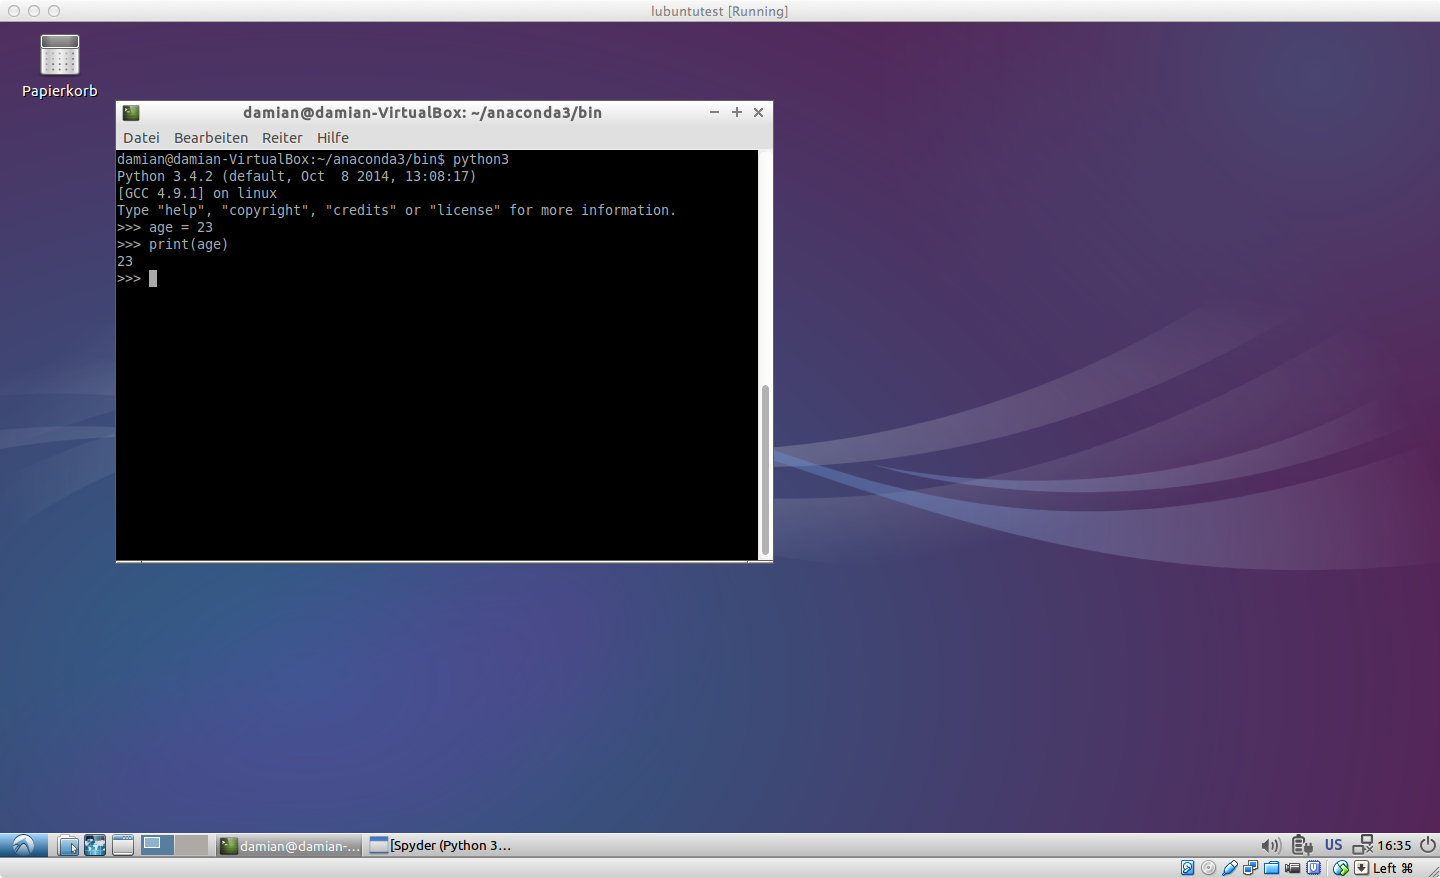
\includegraphics[width=.6\paperwidth,,keepaspectratio]{../pictures/screenshot-terminal} 
	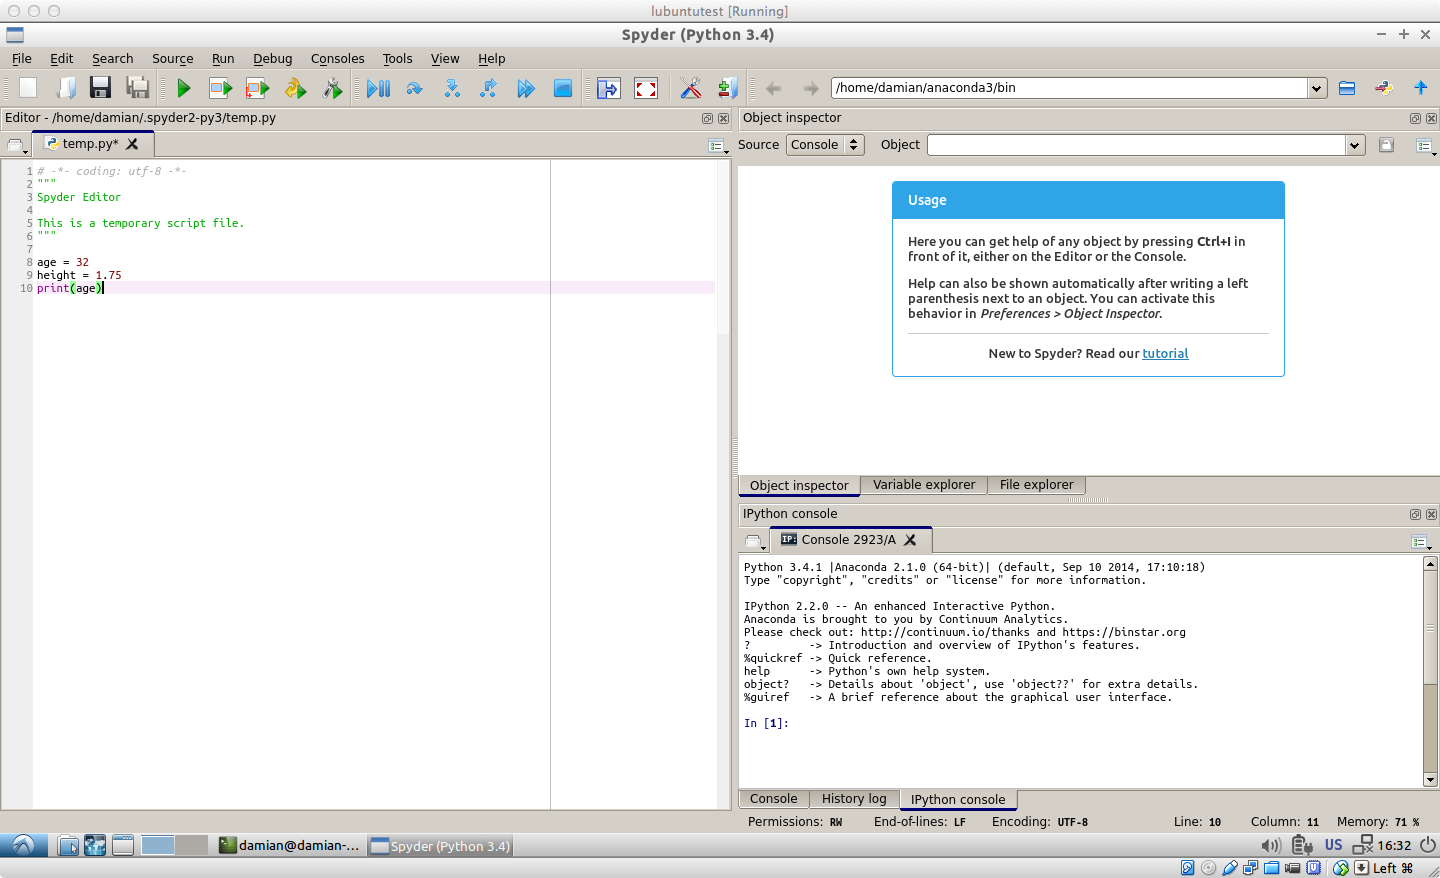
\includegraphics[width=.6\paperwidth,,keepaspectratio]{../pictures/screenshot-spyder}
	\caption{\label{fig:spyder}Different ways to issue Python commands: By starting the interpreter \texttt{python3} in the terminal (top) or by using an integrated development environment (IDE) like spyder (bottom).}
\end{figure}



\section{Integrated development environments (IDE)}

For daily work, though, there are more helpful ways of developing Python code, so called integrated development environments, or IDEs. We will use Spyder, which is very similar to programs you are familiar with. It looks very much like RStudio and a bit like STATA, so you probably feel a bit at home here.

Just start it like this (or by clicking on it in the menu):

\begin{lstlistingbash}
spyder3 &
\end{lstlistingbash}

It is a good environment to work in, and you will probably do a lot of your work in there. There are other IDEs, most notably one called PyCharm, which I use a lot. It is, however, much more geared towards professional programming and less towards data analysis, so you probably do not want to use it at the start of your Python journey.

 
\section{Jupyter Notebook}
\label{sec:jupyter}
Especially for data \emph{analysis}, there is a fourth form of issuing Python commands: Jupyter Notebook, formerly known as iPython notebook. It uses the aforementioned iPython, but lets you run it in your web browser. The great advantage is that you can interactively play with the data, and save code \emph{and} output as well as own annotations in one place. You can find some examples for such notebooks here: \url{https://github.com/damian0604/bdaca/} 

You can start Jupyter Notebook from the command line:

\begin{lstlistingbash}
jupyter-notebook 
\end{lstlistingbash}

It should automatically open a web browser, and lets you do everything from there. For example, in Figure~\ref{fig:jupyter}, you see part of a VAR time-series model conducted in Jupyter notebook.

While this is great for \emph{interactively analyzing} data and keeping track of the output, you might already guess that using Jupyter Notebook is not such a smart way for running programs that take a while to run. For example, if you write a program that downloads a lot of data from websites, maybe running for half an hour or so (as we will do in Chapter~\ref{chap:scraping}), you don't want to do that in your browser. But for statistics stuff like we'll discuss in Chapter~\ref{chap:statistics}, it is really great. For more examples, have a look at the books by \cite{McKinney2012} and \cite{Russel2013}. 



\begin{figure}[h!]
	\centering
	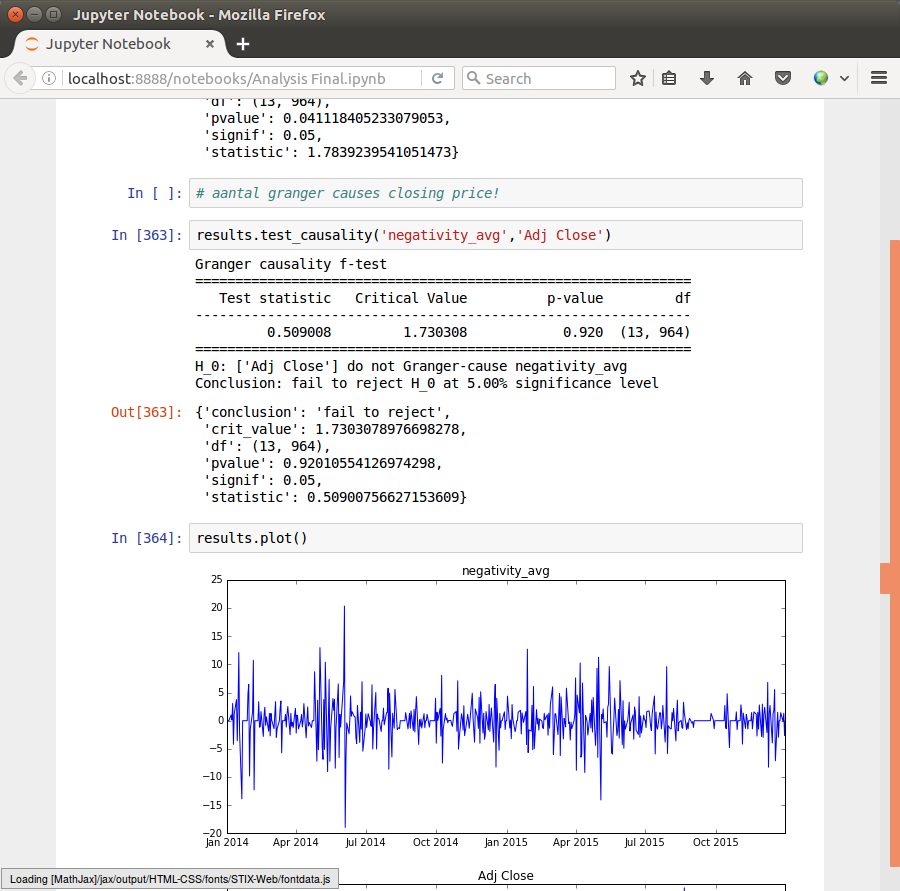
\includegraphics[width=.65\paperwidth,,keepaspectratio]{../pictures/jupyternotebook} 
	\caption{\label{fig:jupyter}Jupyter Notebook lets you run Python code from within your web browser and lets you save it together with the output and your own comments.}
\end{figure}


\section{Recap}
You should have understand why there is no \emph{one} way of ``running Python'' and know what the pros and cons of different ways of running Python code are. 

For you, the most important ones are:

\begin{itemize}
	\item Spyder as an allround solution for daily work
	\item Jupyter Notebook as a useful tool specialized in interactive exploration and analysis of data
\end{itemize}
 
And next to that, you should keep in mind that one can also run programs from the command line or starting an interactive Python interpreter on the command line. There will be a point in time when you want to do that.

 
 
 
\chapter{The very, very basics of programming in Python}
\label{chap:basics}
Before we start writing our first own program, we need to clarify a few concepts. Luckily, they are pretty simple---but nevertheless, it is crucial to completely understand them. 

\begin{quote}
Of course, what I present here is far from complete. I'll mention only the most essential parts that you need to understand to get started. Everything that is not strictly necessary right now or that is pretty intuitive (I guess I don't have to say that mathematical operators like $+$, $-$, $*$, or $/$ work exactly as you'd expect?) will be left out, and a lot is pretty much simplified. That's because our main objective is to get started as soon as possible with some real life data, not to get every detail right as you would do in a computer science course. After all, we are no computer scientists.  
\end{quote}

So, start an environment of your choice (see Chapter~\ref{chap:waystorunpython}) and follow me along with some examples.


\section{Datatypes}
\label{datatypes}
\subsection{Basic types}
When thinking of a \emph{variable}, most social scientists immediately think along the lines of how the term `variable' is understood in SPSS or STATA datasets (or in methods sections in social science papers, for that matter): Something like age that has one value for each case (each person, each newspaper article, each unit of analysis). That's \emph{not} how we define a variable here. (R users might suffer less from this misunderstanding.)

Instead, we distinguish several types of variables (datatypes), and the basic ones take–––in contrast to what you might expect from the SPSS/STATA world---\emph{one and only one} value:

\begin{lstlisting}
age = 33
height = 1.75
male = True
name = "Damian"
\end{lstlisting}

It is of crucial importance to understand that each of these four variables is of a different type. The first one, age, is an \emph{integer}, or, shorter, an \emph{int}: A whole number without anything behind the comma. If age is an int, then someone cannot be aged 32.3. 

The second one, height, is a \emph{floating point number}, or, shorter, a \emph{float}. In contrast to an int, a float can have something behind the comma. Unlike in SPSS, you do not have to specify a number of decimal places, $height=1.7527647326573265743648$ would be perfectly acceptable.

The third one, a \emph{Boolean value}, or, shorter, a \emph{bool}, can only take two values: True or False. Note that there are no \texttt{" "} around True and that True starts with a capital latter. This is how Python recognizes it is not a \ldots

\ldots \emph{string}, the fourth data type. A string contains some arbitrary text, which is indicated by surrounding \texttt{" "} or \texttt{' '}.

\subsection{Type conversion} 
Python automatically converts some types for you (for example, luckily, you can divide a float by an int without thinking about their types). But still, you have to be very careful in using the right datatype. For example, you cannot write code like this:
\begin{lstlisting}
numberofguests = "20"
bottlesofbeer = 100
bottlesperperson = bottlesofbeer / numberofguests
\end{lstlisting}
This does not work, because you cannot divide an int by a string. However, one can convert a string to an int (if the string contains a number):

\begin{lstlisting}
bottlesperperson = bottlesofbeer / int(numberofguests)
print(bottlesperperson)
\end{lstlisting}
This code would work! By the way, if you want to have it the other way around and make a string from an int, the function is called \texttt{str()}.
\begin{quote}
You might wonder why one would have to convert types at all. Couldn't one just use the right type from the start? That's because a lot of data that we will analyze does not come in the right format. For example, if we have a file with some tweets followed by the number of retweets they received, then data that we read from the file in principle is text, thus, a string. If we want to do some calculations with the number of retweets, we have to convert it to an int.
\end{quote}


\subsection{Lists and dicitonaries}
Imagine we want to calculate the mean age of a group. It would be very inefficient to have a variable for every single person:

\begin{lstlisting}
age1 = 22
age2 = 25
age3 = 23
age4 = 28
age5 = 26
meanage = (age1 + age2 + age3 + age4 + age5) / 5
print(meanage)
\end{lstlisting}
In fact, we could almost do it more efficiently by hand. Thus, we might want to have something that is more like what is called a variable in SPSS or STATA: something named age that can contain multiple values. 
Such a datatype is called a \emph{list}. You can have lists of strings, lists of floats, lists of ints, and even lists of lists (and lists of lists of lists\ldots). A list is denoted by \texttt{[ ]}, and the entries are seperated by commas. 
Let's create a list of ints:
\begin{lstlisting}
age = [22, 25, 23, 28, 26]
\end{lstlisting}
To calculate the mean age, we could now divide the sum of the elements by the number of elements (or, technically speaking, by the \emph{length} of the list). We'll discuss such functions in the next section, but for those who cannot wait, this is how it works:
\begin{lstlisting}
age = [22, 25, 23, 28, 26]
meanage = sum(age)/len(age)
print(meanage)
\end{lstlisting}
\begin{question}
What do you think, of what type are \texttt{age}, \texttt{sum(age)}, \texttt{len(age)}, and \texttt{meanage}? If you want to know if you got it right, you can get the answer with \texttt{type(meanage)}, \texttt{type(sum(age))} and so on.
\end{question}
We can also access a specific item from a list: If we want to know the age of the third person, then we can get it with
\begin{lstlisting}
age[2]
\end{lstlisting}
Yes, 2, because we start counting with zero\footnote{If you are in a nerdy mood, you can have a look at this classic (brief) text from 1982 explaining why: \url{http://www.cs.utexas.edu/users/EWD/transcriptions/EWD08xx/EWD831.html}}!
The drawback of our current approach is that you have no idea who the person is that is 23 years old. You could have a second list in the same order:
\begin{lstlisting}
name=["John","Bas","Anne","Sheila","Mark"]
\end{lstlisting}
Note that this is a list of strings, as we can see from the \texttt{"}-signs. Having multiple lists in a corresponding order is actually a strategy we will work with pretty often, and it is pretty much the same as having a dataset with multiple variables in SPSS or STATA. If we are interested in the name and age of the i\textsuperscript{th} person, we could now find out:
\begin{lstlisting}
i=3
print(name[i])
print(age[i])
\end{lstlisting}

Another option would be the last data type that we will discuss: a \emph{dictionary}. As the name says, a dictionary is something where you can look something up–––in Python terms, you search for a \emph{key} and get its \emph{value}. A dictionary is denoted by \texttt{\{ \}}, with entries separated by commas, and keys and values by a colon:
\label{whatsadict}
\begin{lstlisting}
nameage={"John": 22, "Bas": 25, "Anne": 23,"Sheila": 28 ,"Mark": 26}
\end{lstlisting}
Note that in this examples, the keys are strings and the values are ints, but they could also have any other data type.
If we want to know how old Sheila is, we can retrieve that information:
\begin{lstlisting}
print(nameage["Sheila"])
\end{lstlisting}


\section{Functions}
We have played around a bit with variables. To do some useful things with them, however, we need something called \emph{functions}. In fact, we already used some: \texttt{print()} for example, or \texttt{len()} and \texttt{int()}. 
You can imagine a function as a command that in most cases takes some input (or, as we will call it, one or more \emph{arguments}) and does something with it. The  argument is supplied between \texttt{()}. For example, the function \texttt{print()} takes some variable as argument and show its content on the screen. This works for all types you know until now:
\begin{lstlisting}
answer = 42
question = "What's the answer?"
print(question)
print(answer)
\end{lstlisting}
Note that you can use single quotes inside a string if you use double quotes outside the string (or vice versa!), but don't mix them up, otherwise it is unclear where the string ends. 
Of course, you do not have to define the variable in advance but also can do so on the fly:
\begin{lstlisting}
print("Hello world")
\end{lstlisting}
Pay attention to the \texttt{" "}, which indicate that you do not supply a variable name that refers to a string, but the string itself. You could as well write:
\begin{lstlisting}
hi="Hello world"
print(hi)
\end{lstlisting}
This gives exactly the same result.
Another function that we already used is \texttt{len()}. It gives the length of an object, for example, the number of elements in a list or the number of characters in a string. You can actually also use functions within a function: 
\begin{lstlisting}
hi="Hello world"
print("The string",hi,"has",len(hi),"characters")
opdetap=["Estaminet","Steenbrugge Blond","Palm"]
print("They serve",len(opdetap),"different beers")
\end{lstlisting}
Make sure you understand where a \texttt{"} is placed and why!

\subsection{Writing your own functions}
There are a lot of useful functions available, either directly or from one of the numerous additional modules that can be loaded into Python. However, you can also write your own functions. This is something you might not need right now, but it can come in very handy later on. Imagine you would want to write a function to calculate the mean age, given a list of integers with ages. Then you could define a function to do this:

\begin{lstlisting}
def averageage(agelist):
    y = sum(agelist)/len(agelist)
    return y
\end{lstlisting}
We basically define that our function takes some list as input (we  called it \texttt{agelist}, but we could have chosen any other name). Then, it calculates some variable \texttt{y} (again, an arbitrary name) and returns that value.


So, if we have a list
\begin{lstlisting}
ages = [22, 25, 23, 28, 26]
\end{lstlisting}
we can now simply write
\begin{lstlisting}
averageage(ages)
\end{lstlisting}
to get the mean age, because we have defined the new function \texttt{averageage} before.

Obviously, for such a simple thing, this is not really necessary, because we could have just calculated
\begin{lstlisting}
sum(ages)/len(ages)
\end{lstlisting}
directly. But if the calculation is more complicated and if we have to do it repeatedly, this can save us a lot of copy-pasting and makes our code more readable.


\begin{quote}
Once I was teaching this course, a student had the idea of writing a function she named \texttt{translatetoenglish()}. It took a Dutch string as argument, passed that one to to Google Translate, and returned the English translation. So, once the function was defined, you could write something like \texttt{print(translatetoenglish("Wat een mooie dag!"))}, which would produce the following output: \texttt{What a beautiful day!}. She used it for more serious business, namely to loop over a dataset of multilingual tweets to produce a new dataset in English. What a loop is, is explained in Section~\ref{sec:forloops}.
\end{quote}


\section{Methods}
We have learned that a function is called\footnote{To 'call a function' means to execute it.} by simply writing its name and passing some variables as an argument between \texttt{()}. Another way of doing something with variables is using a \emph{method}\footnote{Strictly speaking, a method is also a function, but hey, this is no computer science course, so we'll allow ourselves to be a bit sloppy (and it relieves me from the burden to explain to you what a \emph{class} is, what I would have to do to tell you the complete story).}. In contrast to a function, a method is directly associated with a variable. For example, each string has a built-in method with the name \texttt{.lower()}. If you want to change all Capital Letters to lowercase, you can simply call the method by attaching it to the string. See these examples:
\begin{lstlisting}
hi="Hello world OUT THERE"
print(hi.lower())
print("TESTtttt".lower())
\end{lstlisting}
As you see, methods are very similar to functions, but the way they are called is different. If \texttt{lower()} was a function, you would write \texttt{lower("TEST")} --- but it is a built-in method of each string rather than a function, so you have to call it by writing \texttt{"TEST".lower()} instead. Obviously, \texttt{.lower()} does not need an additional argument to convert the string to lowercase, as it a method \emph{of the very string it is supposed to work on}, so there is simply nothing between the \texttt{()}. Nevertheless, you cannot leave away the\texttt{()}, because every function and every method has to end with \texttt{()}, otherwise, it would not be executed.

For now, it is not important to know why some things are a method and some are a function.\footnote{In fact, sometimes this is kind of an arbitrary choice made by those who invented Python. Some operations have even been implemented as both function and method.} It is important to know, however, that both ways of doing something with your variables exist and how you use them.

\begin{quote}
	Note that functions and methods usually do not change the value of an argument itself but rather return a new object as result. So, if you have a string \texttt{mystring = 'HELLO'}, then calling \texttt{mystring.lower()} does \emph{not} change mystring itself -- it only \emph{returns} the lowercased version of it. You therefore have to assign the result to a new variable (\texttt{mylowerstring = mystring.lower()}) or to the old one (\texttt{mystring = mystring.lower()}).
\end{quote}

\section{For loops}
\label{sec:forloops}
All these functions and methods are mainly interesting if you do not apply them one time, to one string, but hundreds, thousands, or millions of times. In fact, this is the very essence of what we are doing in this course: Splitting up a task in small functions or methods that we then apply repeatedly. 

To tell the computer to repeat something, we use a construction called a loop, or more specifically, a \emph{for-loop}. Let's start with an example (when typing it over, start line 3 by pressing SPACE four times):

\begin{lstlisting}
alltweets = ["Great lecture at the UvA", "I HATE YOU!", "I want BEER"]
for tweet in alltweets:
    print(tweet.lower())
\end{lstlisting}

\begin{quote}
After a line ending with a colon, Python expects an indented block. If you do not do this in a consequent way (for example, you sometimes press TAB, sometimes use 4 spaces, sometimes 3, or none at all, Python will complain and give you an ``indention error''. Some IDEs and some editors automatically convert TABs to spaces, but to avoid any confusion, the best convention is to simply never press TAB and always use spaces.
\end{quote}
What happens? In line 1, we define the list \texttt{alltweets}. In line 2, we instruct the computer to take the first element of the list \texttt{alltweets} and give that element the name \texttt{tweet}. This is done by using the \texttt{for}-command. In human language, it might read as ``Please repeat the task I will explain in the following indented lines \texttt{for} each element \texttt{in} the given list. In the task description given in the following block of indented lines, I will refer to the element that you are working on at that time as \texttt{tweet}''.  

Note that the name  \texttt{tweet} is completely arbitrary chosen, while \texttt{for} and \texttt{in} are mandatory statements.

The indented line, line 3, is now executed. \texttt{tweet} now has the value of the first tweet of the first element of \texttt{alltweets}. After the indented block is finished, the program goes back to line 2, takes the next element from the list, assigns the name \texttt{tweet} to that next element, executes the indented block, and repeats until all elements have been used.

We could extend our code to produce output that looks a bit more fancy (and do not forget to indent lines 4 to 7 by using four spaces at the beginning of each line):

\begin{lstlisting}
i=0
alltweets = ["Great lecture at the UvA", "I HATE YOU!", "I want BEER"]
for tweet in alltweets:
    print("Printing tweet number",i,"in lowercase:")
    print(tweet.lower())
    print("\n")
    i = i +1
\end{lstlisting}

\texttt{\textbackslash n} denotes a line ending, so we get an empty line. In the last line, we add one to our counter variable \texttt{i}. A short form of doing this is \texttt{i+=1}, and it's pretty likely that I'll use that shorthand in the lectures.

\begin{question}
Can you write your own loop based on the functions and data structures you learned until now?
\end{question}


\section{If statements}
Another important way of structuring your code is to define that it only has to be executed under specific conditions. Again, the block of code that has to be executed under a condition is indented and introduced by a colon.

\begin{lstlisting}
age = 23
if age > 25:
	print("Older than 25")
\end{lstlisting}

Of course, this does not print anything, as 23 is less than 25. You can also specify different conditions using the \texttt{elif} statement:

\begin{lstlisting}
age = 23
if age >23:
	print("Older than 23")
elif age <23:
	print("Younger than 23")
elif age==23:
	print("Exactly 23")
\end{lstlisting}

If you want to have a condition that is met if none of all others are met, you can use \texttt{else:}.
Note the double == in line 6. This is very important: a single = assigns a value to a variable, a double == compares two variables. Maybe it is obvious, but also note that you can nest such structures and have a condition within a for-loop (and maybe have another loop within the condition). 

\begin{question}
Can you write a program that takes each element from a list (using a for-loop), and then prints it if it if satisfies a specific condition?
\end{question}

\section{Recap}
You should have no problems explaining what the following datatypes are:
\begin{itemize}
\item int
\item float
\item bool
\item string
\item list
\item dictionary
\end{itemize}

You should know what functions and methods are and how to use some basic ones like \texttt{print()}, \texttt{len()} or \texttt{.lower()}.

You should have understood that you can write such functions yourself.

And, very importantly, you have to understand for-loops and if-conditions, including the role of indentation to structure your code.


\chapter{Retrieving and storing data}
We already learned in section \ref{datatypes} (\nameref{datatypes}) how we can internally create some data structures that we can use to further do some analyses. For example, if we wanted to do some analyses with names, ages, and height, we could create three lists like this:

\begin{lstlisting}
age = [22, 25, 23, 28, 26]
name = ["John","Bas","Anne","Sheila","Mark"]
height = [1.83, 1.77, 1.55, 1.76, 1.74]
\end{lstlisting}

But of course, if we had such a limited amount of data, we wouldn't need to write a program to analyze it. So, we probably want to import the data from an external source. In this chapter, we will describe some ways to to this.


\section{CSV files}

In the easiest secenario, we already have a \emph{table} in which each row contains a case and each column the value for age, name, and height, respectively. The universally acceptable format for such a table are CSV files: Text files in which columns are seperated by commas. Sometimes, a semicolon is used instead,  conventions differ. Others use a TAB character instead, which is essentially the same, although one usually calls it a TAB-seperated file then.

You actually already saw a CSV file on page \pageref{firstcsvfile}. Have a look back there if you forgot. Virtually all programs (including SPSS, Stata, Excel, \ldots) can read and write CSV files, that's why we will use them very frequently. When creating data with such a program, make sure that you know how they are formatted exactly (e.g., are columns separated by \texttt{,} or \texttt{;}, are strings encapsulated by \texttt{""} or not, \ldots. You can use the tools described on page~\pageref{firstcsvfile} to inspect the files.

Lets create a text file with the following content:
\begin{lstlistingoutput}
John,22,1.83
Bas,25,1.77
Anne,23,1.55
Sheila,28,1.76
Mark,26,1.74
\end{lstlistingoutput}

You can use gedit for this, an editor you find somewhere in the menu, but which you can---surprise, surprise!---also start from the command line with \texttt{gedit~\&}. Let's assume we saved this file as \texttt{/home/damian/mensen.csv}.

Now we can write a simple Python program to read this data:
\begin{lstlisting}
import csv
name=[]
age=[]
height=[]
with open('/home/damian/mensen.csv', encoding='utf-8',mode='r',newline='') as csvfile:
    reader = csv.reader(csvfile, delimiter=',')
    for row in reader:
        name.append(row[0])
        age.append(row[1])
        height.append(row[2])
print("Done!")
\end{lstlisting}
We see a lot of familiar structures: for example, the construction of (empty) lists in lines 2 to 4, the \texttt{for}-loop in line 7 to 10. So, let's first focus on the new parts:
\begin{itemize}
\item The \texttt{import} statement. It simply says that we want to load an external module, in this case one that knows how to read csv files. Import statements are usually written in the very first lines of a python scripts.
\item The \texttt{with open(\ldots) as:} construction. It indicates that we want to open a file and assigns a name to that so-called \emph{file object}, indicated by \texttt{as} (in this case, we decided to call it \texttt{csvfile}, which is a completely arbitrary name). The statement ends with a colon, so an indented block has to follow (remember?). When the indented block is over (thus, after line 10), the file is automatically closed again. That's exactly what we want, because by then, we have read all the information and stored it in lists; we don't need the file any more. The arguments passed to the \texttt{open()} function specify the file name, but also some other details of how to open it. We'll skip the details for now.
\item The \texttt{csv.reader()} function. It returns an object\footnote{For those who are interested: More specifically, it returns a so-called generator. You can loop over a generator, but you can do so only once. In every iteration of the loop, it gives you one next element (one more row from the file in our case), and once there are no elements left, it stops. The great advantage of this, especially when dealing with large files, is that you don't have to load the whole file into memory at once.} (which I decided to call, not very creatively, \texttt{reader}) that we can use to actually read the file. Note that in line 5, we only \emph{opened} the file, we have not \emph{read} a single byte from it yet. In line 5, we actually could have opened any arbitrary file---the \texttt{open()} command does not imply a specific data structure. Therefore now, in line 6, we define how to read from the file: Namely, by using the \texttt{csv} module. As an argument, we can give more specific information, for example, as done here, that the columns are separated by a \texttt{,}.
\item The \texttt{.append()} method. It adds a new element to a list.
\end{itemize}

With your knowledge gained so far, you probably already can explain what in the for-loop in line 7--10 exactly happens. Think about it for a moment before reading further.

OK, the solution.

In line 7, we take the first row from the csv table, as provided by the \texttt{reader} object. We call it row. \texttt{row} simply is a list of all columns in that specific row. So, when we start, it is the list \texttt{["John",22,1.83]}. This means that we can get the value in the first column, \texttt{"John"}, by asking for the first element of the list, namely \texttt{row[0]}. That's what we do in line 8, where we put this value into the (until now empty) list of \texttt{name}s. The same is done with age and height, before we return to line 7 and get the next row from the \texttt{reader}. 

Now, \texttt{row} has the value \texttt{"Bas",25,1.77}, and we again append \texttt{row[0]} to the list \texttt{name}, \texttt{row[1]} to the list \texttt{age}, and \texttt{row[2]} to the list \texttt{height}. We continue with this procedure until nothing is left to read from the file. 

Let's also check if the data actually looks like what we expected:
\begin{lstlisting}
print(name)
print(age)
print(height)
i=2
print(name[i],'is',age[i],'years old and',height[i],'meter tall')
\end{lstlisting}
Great! 

Let's now save these columns in to a new file, \texttt{test.csv}, but in a different order. To this end, we use the \texttt{zip} command that basically glues several lists together. It goes like this:

\begin{lstlisting}
output=zip(age,height,name)
with open("test.csv",mode="w",encoding="utf-8") as fo:
    writer=csv.writer(fo)
    writer.writerows(output) 
\end{lstlisting}

That's all! Have a look at the file you just created and check if everything went right.

\section{JSON files}
\label{json}
OK, let's do this quickly, because what we will do in the next section is way cooler: We will retrieve JSON-data directly from an Google or Twitter. JSON is a data structure that is very similar to (if not identical to the one of) a Python dict, You already learned on page \pageref{whatsadict} what a dict is. Have a look back if you do not recall exactly.

Because a JSON file has the same data structure, we can open a JSON file and directly import it into a dict. This is really handy, as a lot of online data is available in that format.

Lets again (with an editor like gedit) create a file with the following content and call it \texttt{/home/damian/mensen.json}.
\begin{lstlistingoutput}
{"Sheila": 28, "Anne": 23, "John": 22, "Bas": 25, "Mark": 26}
\end{lstlistingoutput}

To read this file into a Python dict, we only need to do the following:
\begin{lstlisting}
import json
with open("/home/damian/mensen.json", mode="r", encoding="utf-8") as fi:
        mydict = json.load(fi)
print(mydict)
print("Sheila is",mydict["Sheila"])
\end{lstlisting}
Note that  both the dictionary name \texttt{mydict} and the name of the file object \texttt{fi} are completely arbitrary. I often use \texttt{fi} (file in) for files I read from and \texttt{fo} (file out) for files I want to write to, so that I don't confuse the two.

As you might expect, saving is as easy as opening. We only need to do call the function \texttt{json.dump()}, which takes two arguments: the dictionary that we want to save and a file object:
\begin{lstlisting}
import json
ages = {"Sheila": 28, "Anne": 23, "John": 22, "Bas": 25, "Mark": 26}
with open("/home/damian/mensen.json", mode="w", encoding="utf-8") as fo:
        json.dump(ages,fo)
\end{lstlisting}
Note that in the \texttt{open()} function, we now specify \texttt{mode="w"} instead of \texttt{"r"} --- we open a file for writing, not for reading.
\begin{quote}
Note that opening a file for writing (i.e., with \texttt{mode="w"}) creates a new file if it does not exist, \textbf{but if it already exists, it immediately deletes all content} that might have been in there.
\end{quote}

But as I promised, it get's cooler, because in the next section, we will retrieve JSON objects not from a file, but directly via an API.

\section{APIs}
\subsection{How does it work?–––A first example}

\begin{figure}[h]
\centering
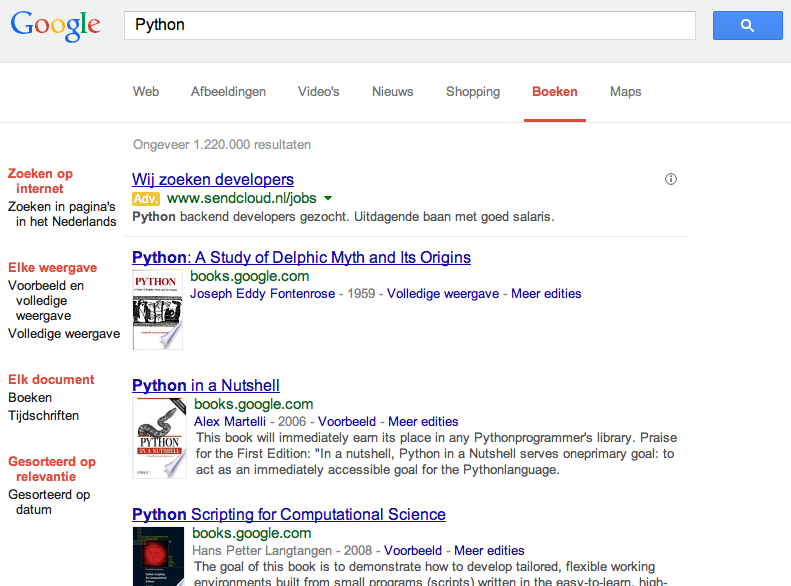
\includegraphics[width=.6\paperwidth,,keepaspectratio]{../pictures/screenshot-googlebooks}
\caption{\label{fig:googlebooks}The GoogleBooks web interface}
\end{figure}

Let's assume we want to retrieve data from some online service, for example book descriptions from GoogleBooks. Of course, we could surf to their website, enter a search query, and somehow save the result. This would result in a lot of impracticalities, most notably that the website is perfectly readable and understandable for humans, but may have no meaning for a computer program. As humans, we have no problem understanding which parts of Figure~\ref{fig:googlebooks} refer to the author of a book, what the numbers "2006" and "2008" mean, and on. But it is not trivial to think of a way to explain to a computer program how to identify variables like \texttt{author}, \texttt{title}, or \texttt{year} in the output. 
\begin{quote}
We will learn how to do exactly that in Section \ref{parsing} (\nameref{parsing}). Writing such a parser can be really useful, but it is also error-prone and some kind of a detour, as we are trying to bring some information that has been optimized for human reading \emph{back} to a more structured data structure. Thus, if an API exists, it saves \emph{a lot} of work. 
\end{quote}

Luckily, however, many online services do not only have web interfaces, but also offer another possibility to access the data they provide: an API (Application Programming Interface). In our example, we submit our request to GoogleBooks, and the API returns a JSON object with all the relevant data in it, in a neat and organized structure.

Consider the case of GoogleBooks. It offers an extremely simple API, as you do not have to log on (everyone can just use it), and because you call it in a very straightforward way: Assiming that you want to retrieve books that match the search string "python", you simply open the url \url{https://www.googleapis.com/books/v1/volumes?q=python} --- and get a JSON object with all relevant information.

\begin{lstlisting}
from urllib.request import urlopen
import json
from pprint import pprint
antwoord=urlopen("https://www.googleapis.com/books/v1/volumes?q=python").read()
data=json.loads(antwoord.decode("utf-8"))
pprint(data)
\end{lstlisting}
What does the code do? In lines 1 to 3, we import a module to download data from a URL, a module to read JSON data, and (to have some luxury) a module that prints json objects in a more readable way. Nothing spectacular so far.

In line 4, we access the GoogleBooks API and store the response in a variable we gave the arbitrary name \texttt{antwoord}. The function \texttt{urlopen} opens the URL, and its \texttt{.read()} method actually reads the content one gets when accessing the URL. Note that this is very much the same like opening a file and subsequently reading its content.

Until now, \texttt{antwoord} is just a bunch of bytes, and we have not made any attempt to somehow interpret it. That's what we do in line 5: \texttt{antwoord.decode("utf-8")} transforms the bunch of bytes into a string. However, a string is not really what we want, because we know that the string contains in fact JSON data\footnote{We know these things (that the bytes are a UTF-8 encoded string and that the string contains JSON data) because it is defined like that somewhere in the documentation of the GoogleBooks API. Nevertheless, both things are very common for many APIs, and one could therefore just try it out as well.}. And, as we saw in Section \ref{json} (\nameref{json}), a JSON string can be directly translated to a Python dict. This is done by the function \texttt{json.loads()}. Thus, \texttt{data} contains a Python dict with all information provided by the GoogleBooks API based on our search query. In line 6, we simply print that information.
\begin{quote}
Why \texttt{json.loads()} in line 5 and not \texttt{json.load()}, as we did in Section \ref{json} (\nameref{json})? Because \texttt{json.load()} takes a file object (which we don't have here) as argument, and \texttt{json.loads()} a string.
\end{quote}
 
 	
Let's have a look at the output \texttt{pprint(data)} produced to see what is actually stored in our dict \texttt{data}. As you can see, it is a lot, which is why I removed some lines from the following listing to make the picture clearer.
 
\begin{lstlistingoutput}
{'items': [{'accessInfo': {'accessViewStatus': 'SAMPLE',

<<I REMOVED SOME LINES HERE>>

   'volumeInfo': {'authors': ['Niklas Luhmann'],
         'canonicalVolumeLink': 'http://books.google.nl/books/about/Love.html?hl=&id=Hh-kncGf4QkC',
         'categories': ['Social Science'],
         'contentVersion': '0.0.2.0.preview.3',
         'description': 'This short text, originally '
            
<<I REMOVED SOME LINES HERE>>
            
         'language': 'en',
         'pageCount': 96,
         'previewLink': 'http://books.google.nl/books?id=Hh-kncGf4QkC&printsec=frontcover&dq=inauthor:%22Niklas+Luhmann%22&hl=&cd=1&source=gbs_api',
         'printType': 'BOOK',
         'publishedDate': '2010-12-06',
         'publisher': 'Polity',
         'readingModes': {'image': True, 'text': True},
         'subtitle': 'A Sketch',
         'title': 'Love'}},

\end{lstlistingoutput}
 
First of all, we see at the very beginning that \texttt{data} contains an entry  \texttt{items}, which is is probably what we need. We could access this part of the dict by typing  \texttt{data["items"]}. 

Now let's see what \texttt{data["items"]} consists of. First of all, it seems to be a list of different items (book records, in our case), as \texttt{[} denotes the beginning of a list here (in contrast to \texttt{\{}, which would imply a dict, see Section \ref{datatypes} (\nameref{datatypes})). This implies that we could get the i\textsuperscript{th} book by typing \texttt{data["items"][i]}.

What information is provided for each item? First of all, we find another dict called \texttt{'accessViewStatus'}. This doesn't look very interesting, so let's skip it. Some lines later, however, we see that our first book (and presumably also all the following books) have a dictionary called \texttt{'volumeInfo'}. That looks promising!

Now we're there! The dict \texttt{data['items'][i]['volumeInfo']} consists of several key-value pairs, so that we could get the language in which the 3\textsuperscript{rd} book was written by typing:
 \texttt{data['items'][2]['volumeInfo']['language']}
(remember, we start counting at 0).

\begin{quote}
	If you want to see all keys of a given dictionary \texttt{mydict} without having to wade through all the output, then you can get them by calling the method \texttt{mydict.keys()}.
\end{quote}

Let's put all this into practice and write a small program that gives us some information on books written by a specific author. What about some information on books written by Niklas Luhmann, one of the most important social theorists of the 20\textsuperscript{th} century\footnote{Accoring to Wikipedia. Actually, we could also access Wikipedia's API as well to directly retrieve this information. But, to be honest, I just used their web interface. But if I were to collect biographical information on more than 20 sociologists, it would probably already worth learning how to use Wikipedia's API.}? We just saw how to access the data we retrieve from the API, but we still have to see how we can transmit a more complicated search string (namely, one specifying that we are interested in one author only).
 
Let's do some reverse engineering. By playing around with the GoogleBooks web interface and paying attention to the URLs that appear in your browser's address bar, you can actually infer how the part after \texttt{?q=} is constructed for more complicated search strings. I basically surfed to \url{http://books.google.com}, entered Luhmann as search string, got some results, clicked on the link of one of the results that were actually indeed written by Luhmann, which then gave me the page showed in Figure~\ref{fig:luhmann}. In fact, I saw that entering \texttt{inauthor:"Niklas Luhmann"} would have been the correct search string for what I intended, and I also saw that this indeed becomes part of the URL.
\begin{figure}[h]
\centering
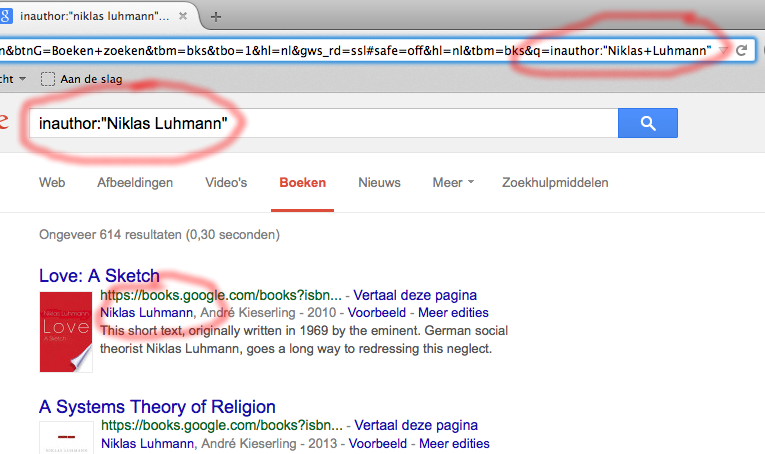
\includegraphics[width=.6\paperwidth,,keepaspectratio]{../pictures/luhmann}
\caption{\label{fig:luhmann}Reverse-engineering the GoogleBooks API}
\end{figure}


Putting all this information together makes it possible to write the following code to retrieve information on  some books written by Luhmann:


\begin{lstlisting}
luhmann=urlopen('https://www.googleapis.com/books/v1/volumes?q=inauthor:"Niklas+Luhmann"').read()
niklas=json.loads(luhmann.decode("utf-8"))
for boek in niklas["items"]:
    print (boek["volumeInfo"]["authors"],": ",boek["volumeInfo"]["title"])
\end{lstlisting}

And why not calculate how long they actually are?


\begin{lstlisting}
totalpages=0
numberofbooks=0
for boek in niklas["items"]:
    pages=int(boek["volumeInfo"]["pageCount"])
    print(pages)
    totalpages=totalpages+pages
    numberofbooks=numberofbooks+1
print ("The average length of a book by Luhmann is", totalpages/numberofbooks, "pages")
\end{lstlisting}


\begin{question}
An alternative way of solving the same problem would be the following program. Can you see advantages and disadvantages of both approaches? Which approach would you choose?

\begin{lstlisting}
pagelist=[]
for boek in niklas["items"]:
    pagelist.append(int(boek["volumeInfo"]["pageCount"]))
print ("The average length of a book by Luhmann is", sum(pagelist)/len(pagelist), "pages")
\end{lstlisting}

\end{question}

\subsection{The Twitter API}
\label{subsec:twitterapi}
For this exercise, we need to import a module named \texttt{twitter}.\footnote{Another popular module for accessing the Twitter API is called \texttt{tweepy}. If you want to dig deeper into using the Twitter API, you might want to check that one out as well and find out which one fits your purposes best.} You can easily install it from the command line with
\begin{lstlistingbash}
sudo pip3 install twitter
\end{lstlistingbash}
Do this before you read any further.

There is a lot of information on the Web, an extensive documentation on \url{https://dev.twitter.com/}, and we will have a number of exercises on the Twitter API in class, so there is no need to go too much into detail here. There are two main differences with the GoogleBooks-example: (1) You do not have to access the API directly via \texttt{urlopen()}, but some nice person already wrote a so-called wrapper which does that for you; and (2) you need an account and log on.


\begin{figure}[h]
\centering
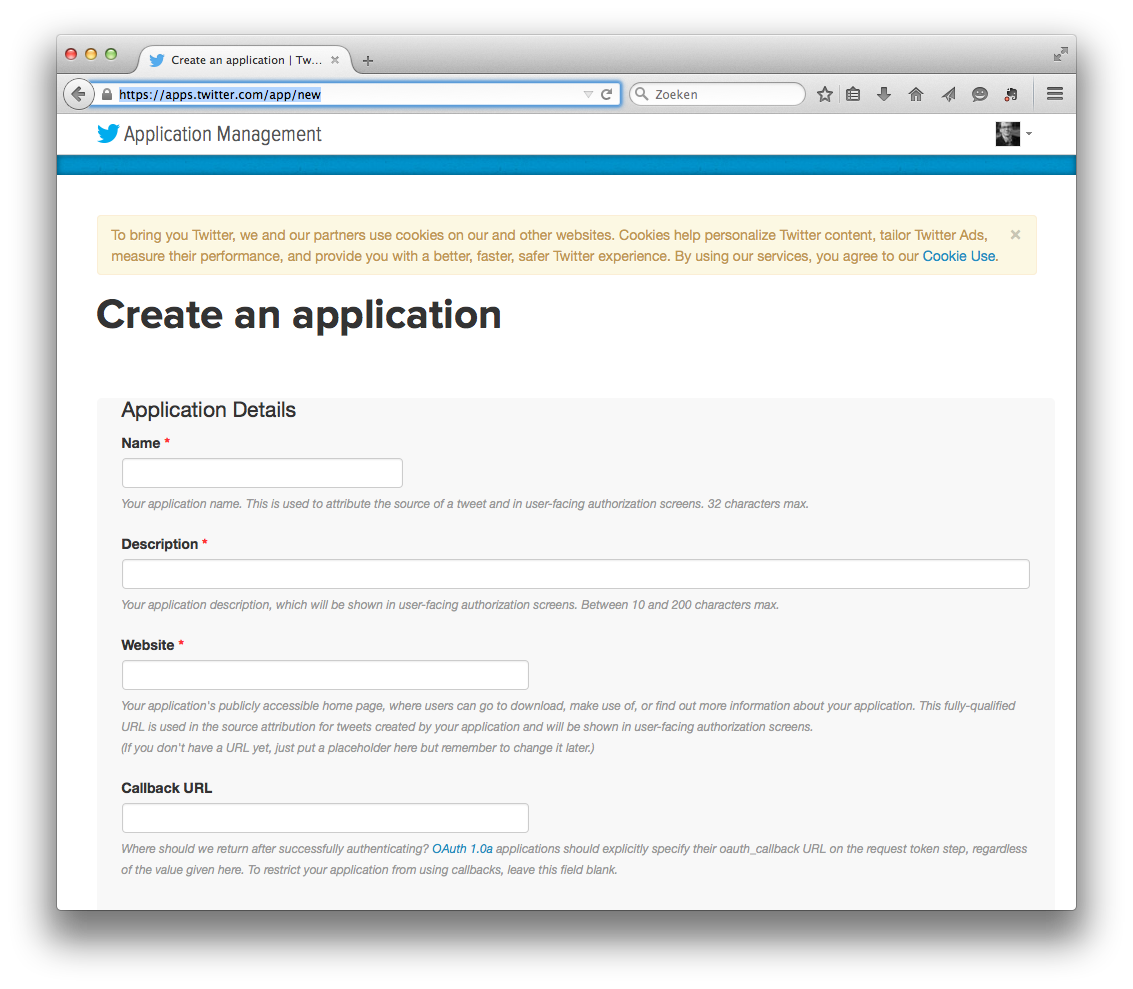
\includegraphics[width=.9\textwidth,keepaspectratio]{../pictures/twitter_createapp.png}
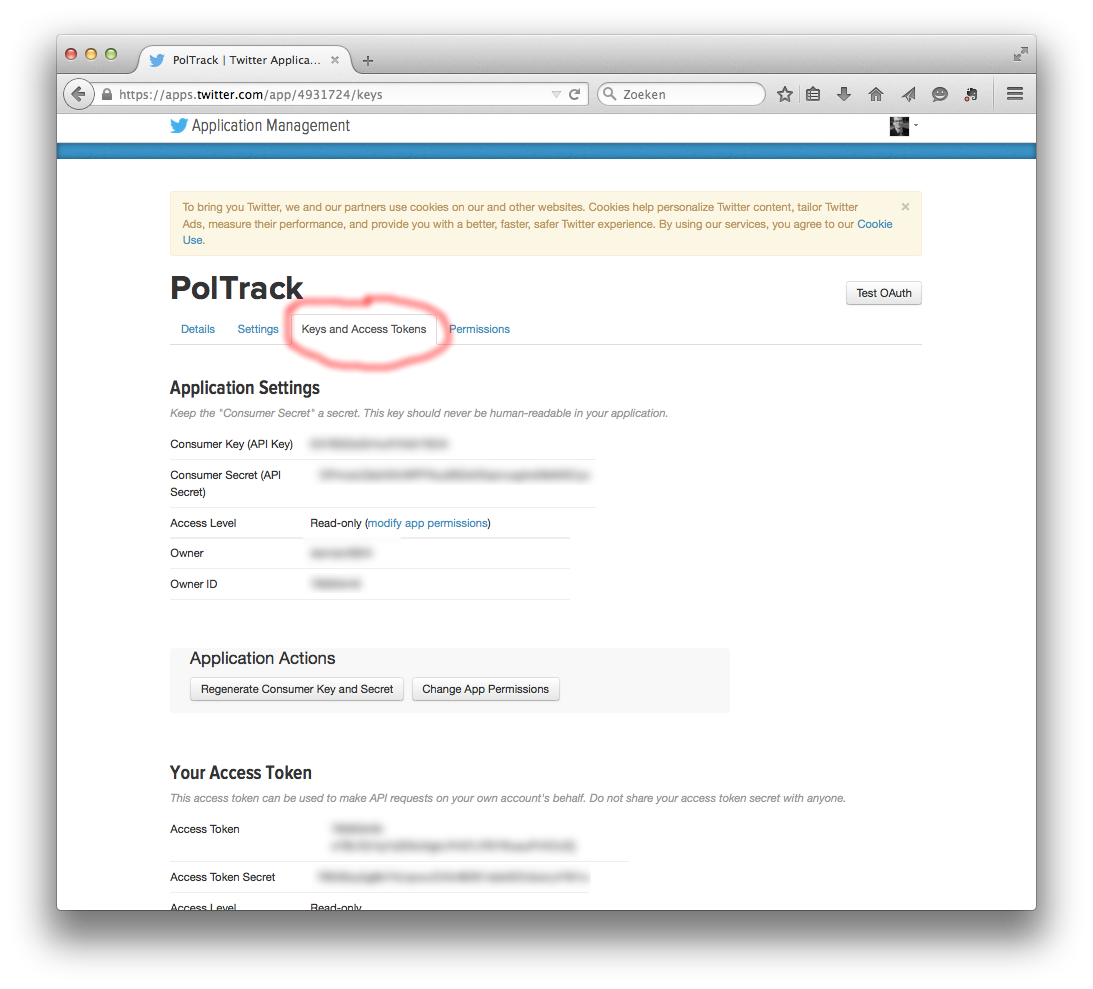
\includegraphics[width=.9\textwidth,keepaspectratio]{../pictures/twitter_createtokens.png}
\caption{\label{fig:twittercreate}Creating a Twitter app and requesting tokens}
\end{figure}

To create an account, go to \url{https://apps.twitter.com/app/new}, register as a developer, create a new app and note down your consumer key, consumer secret, access key and access secret (the latter two are also referred to as access token).  See Figure~\ref{fig:twittercreate} for screenshots. Most things should be rather self-explanatory. You can leave the field for a ``callback URL'' empty, and for ``website'', just make something up like \texttt{idontknowyet.com}. 

In the following example, replace ACCESS\_KEY etc. with your data (don't forget to put them between \texttt{" "}). If you want to retrieve my last 20 tweets as a JSON object (who wouldn't want to do that?), you can simpy do so with a three-line program:

\begin{lstlisting}
from twitter import *
twitter = Twitter(auth = OAuth(ACCESS_KEY, ACCESS_SECRET, CONSUMER_KEY, CONSUMER_SECRET))
posts=twitter.statuses.user_timeline(screen_name="damian0604", count=20)
\end{lstlisting}

If you do not care about my tweets, but rather about more general information about me (like my bio statement or the number of followers I have), you can do so as well:
\begin{lstlisting}
tweep="damian0604"
info=twitter.users.show(screen_name=tweep)
print(tweep,"has",info["followers_count"],"followers.")
print("He is following",info["friends_count"], "people.")
print("This means that his follower-to-following-ratio is",int(info["followers_count"])/int(info["friends_count"]))
print("\nThis is what he says about himself:\n")
print(info["description"])
\end{lstlisting}
To see what type of elements \texttt{info} contains, you can either read the documentation on \url{https://dev.twitter.com/} or use \texttt{print} or \texttt{pprint} to inspect its structure. 

\section{Saving the retrieved data}
Once you have retrieved the data from an API, there are several ways to go. You could directly analyze them in some way, but maybe you just want to save them first (in fact, it might be a good idea to sve them anyway for archiving purposes). Combining our knowledge we gained up til know, we can conceive of multiple ways of storing the data. The first possibility, as we have learned, would be to simply dump the Twitter dataset we aquired into a JSON file.
\begin{lstlisting}
with open("/home/damian/someone.json", mode="w", encoding="utf-8") as fo:
        json.dump(info,fo)
\end{lstlisting}

We could also think of writing a CSV table, in which we store only the relevant information. This is especially useful if we want to further anayze the data using a different program later on. To this end, we could first store all relevant information in lists and then save these lists to a CSV file.


\begin{lstlisting}
import csv
tweets=[]
dates=[]
for p in posts:
	tweets.append(p["text"])
	dates.append(p["created_at"])
output=zip(dates,tweets)
with open("tweetswithdate.csv",mode="w",encoding="utf-8") as fo:
	writer=csv.writer(fo)
	writer.writerows(output) 
\end{lstlisting}




\section{Another example: The AmCAT API}
Some of you might use AmCAT \citep{VanAtteveldt2008}, a framework for content analysis. If you have no idea what AmCAT is, just skip this section. If you do, however, you will be delighted to hear that you can access your AmCAT projects via an API and retrieve all your data for further analysis with Python.

First, you have to install the AmCAT Client:

\begin{lstlistingbash}
sudo pip install amcatclient
\end{lstlistingbash}


You need your username, your password, the project number, and the article set number. Then, you can simply adapt the following sample script to your own needs.

\begin{lstlisting}
import json
import csv
from amcatclient import AmcatAPI

api = AmcatAPI('https://amcat.nl', 'USERNAME','PASSWORD')
articles = api.list_articles(project='XXXX', articleset='XXXX')

# articles is a generator, meaning you can read it only once
# that's impractical for us, so we turn it into a list:
articles = [art for art in articles]

#get an idea about the data by printing info about the first item
print(articles[0].keys())
print(articles[0])

#%% save as json
with open("articles.json",mode="w",encoding="utf-8") as fo:
        json.dump(articles,fo)
 
#%% additionally, make a csv table with some of the data fields
with open("articles.csv",mode="w",encoding="utf-8") as fo:
    writer=csv.writer(fo)
    for art in articles:
        # while saving, make sure that the text does not contain 
        # linebreaks ("\n" or "\r")
        writer.writerow([art["medium"],art["date"],art["text"].replace("\n"," ").replace("\r"," ")]) 
\end{lstlisting}




\section{Recap}
You should have understood 
\begin{itemize}
\item how a CSV file looks like and how it can be read;
\item how a JSON file looks like and how it can be read;
\item how JSON data can be retrieved via an API;
\item how to write the retrieved data to a JSON file;
\item how to write the retrieved data to a CSV file.
\end{itemize}


\part{Specific techniques}
\label{part:specific}

\chapter{Sentiment analysis}
\section{Preparation}
In this chapter, we are going to conduct a sentiment analysis. You can use your own data for this, you only have to modify the proposed code accordingly. For instance, you can use the examples from earlier chapters about how to use CSV files, JSON files, or APIs and add the sentiment analysis code from the examples below to them.

We will discuss several approaches to sentiment analysis below and use several example datasets. In the end, you should be able to transfer what you learned to own datasets and make an informed decision on the approach to use.


You can also download the whole code for the first example if you want to:

\begin{lstlistingbash}
wget https://raw.githubusercontent.com/damian0604/bdaca/master/examples/ex-senti-simple.py
\end{lstlistingbash}


\section{A simple dictionary-based approach}
\label{simplesent}

The simplest way to do a sentiment analysis is to simply count the number of positive and negative words in a text. While this has obvious drawbacks (for example, because we do not care about word order, we cannot distinguish between `good' and `not good'), it is a good starting point to understand how sentiment analysis works. Moreover, because the approach is so simple, you can easily modify it to measure other things.

First of all, we need a list of negative words and a list of positive words. Let's use the command line to make a new directory and download two files with such lists from the internet\footnote{The example presented here is based on the following tutorial: \url{http://nealcaren.web.unc.edu/an-introduction-to-text-analysis-with-python-part-1/}, and the word lists are originally developed by \cite{Wilson2005}}:

\begin{lstlistingbash}
cd /home/damian
mkdir sentiment
cd sentiment
wget http://www.unc.edu/~ncaren/haphazard/negative.txt
wget http://www.unc.edu/~ncaren/haphazard/positive.txt
\end{lstlistingbash}


Let us use some Twitter data to play with. Unfortunately, Twitter does not allow to share datasets with tweets. It does allow, however, to share lists with tweet ids. Via the Twitter API, anyone can then download the whole tweets and reconstruct the dataset.

I prepared a list of tweet ids with tweets about Bernie Sanders in the pre-election period of the US elections before a candidate was nominated. I also prepared a script that automatically downloads the associated tweets.

Download them\ldots
\begin{lstlistingbash}
wget https://raw.githubusercontent.com/damian0604/bdaca/master/examples/sanders.txt
wget https://raw.githubusercontent.com/damian0604/bdaca/master/examples/retrievetweets.py
\end{lstlistingbash}
\ldots and then open \texttt{retrievetweets.py}, where you have to change lines 5 to 8 by entering your API credentials (see Subsection~\ref{subsec:twitterapi}). Now you can run the file, and it will retrieve a set of approximately 900 tweets and save them to a TAB-separated file.

First of all, you should carefully inspect the file to get an understanding of the data structure. For example, you could use the \texttt{head} command on the bash command line (see Chapter~\ref{firstcsvfile}):

\begin{lstlisting}
head -5 sanders.tsv
\end{lstlisting}

Which columns are interesting? Is there a header line (with column names), or do all lines contain data?

Once we have this information, we can make a plan on how to proceed. 
\begin{enumerate}
\item We can skip the header row with the \texttt{next()} function (you didn't know that yet, but now you do).
\item We need a \texttt{list} of all tweets. As we know we can get this by starting with an empty list, followed by looping over all rows in the file and appending the value of the appropriate column to that list.
\item We are only interested in the words, not in punctuation. So, we could make a second list where we replace them by a space. This can be done using the \texttt{.replace()} method. 
\setcounter{lijst}{\theenumi}
\end{enumerate}


\begin{lstlisting}
import csv
tweetlist=[]
processedlist=[]
with open("/home/damian/sentiment/sanders.tsv") as fi:
    reader=csv.reader(fi,delimiter='\'})
    next(reader)
    for row in reader:
        tweet=row[0]
        tweet_processed=tweet.lower().replace("!"," ").replace("."," ").replace("?"," ").replace(u"\u201A"," ").replace("'"," ").replace('"'," ").replace('#'," ").replace(':'," ")
        tweetlist.append(tweet)
        processedlist.append(tweet_processed)
\end{lstlisting}

Ok, we have the data and already did the necessary preprocessing (removing unnecessary characters in this case). BTW: You see why we access the element with the index 0 of the list \texttt{row} in line 7?

You might actually want to have a look at how the data look like to see that you did not make any mistakes. You can do so with some \texttt{print()} functions, or by clicking on the values in the variable explorer (Figure~\ref{fig:inspectvariables}).

\begin{figure}[h]
\centering
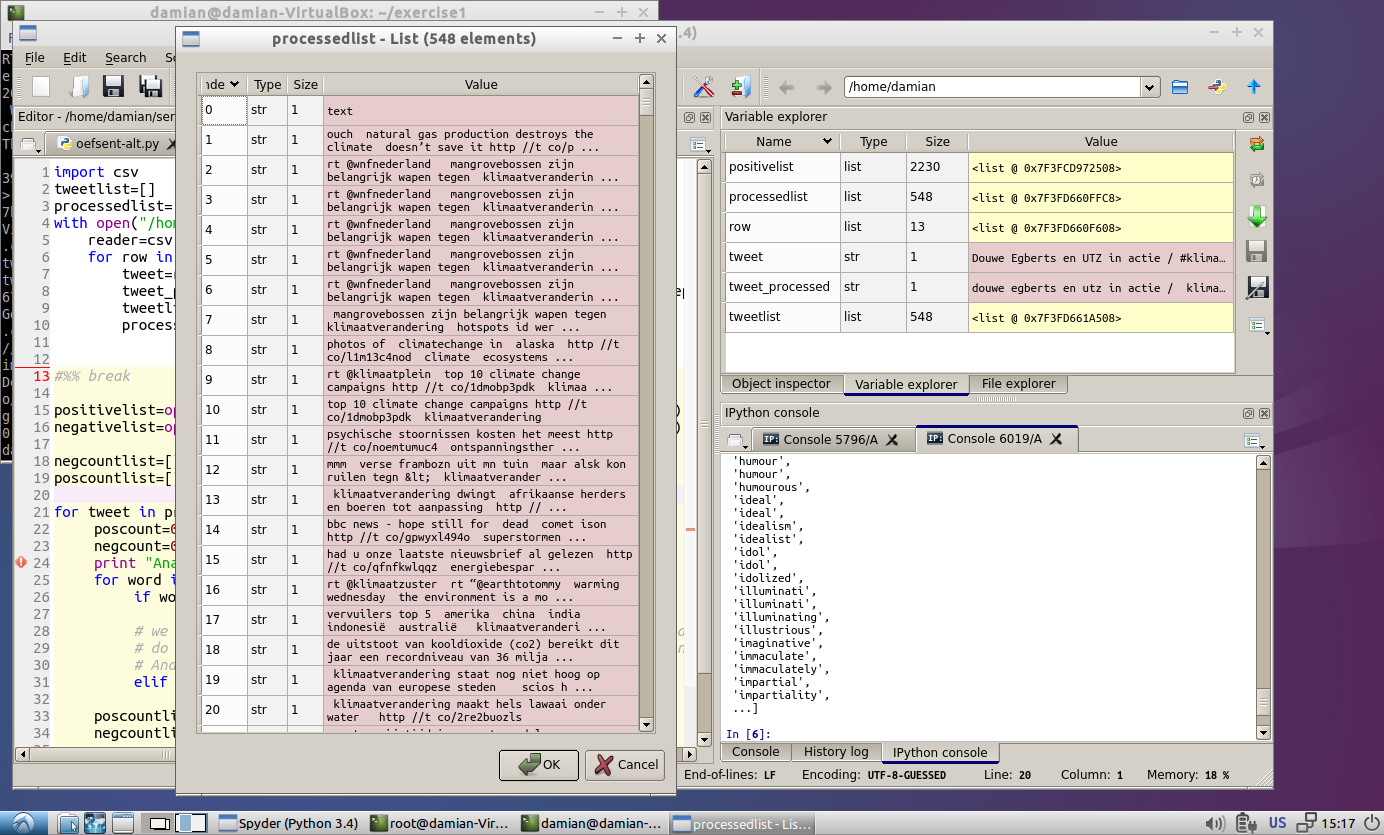
\includegraphics[width=.9\textwidth, keepaspectratio]{../pictures/inspectvariables}
\caption{\label{fig:inspectvariables}Inspecting the data with Spyder's variable explorer}
\end{figure}

We can now plan our next steps:

\begin{enumerate}
\setcounter{enumi}{\thelijst}
\item We need to read a list of positive words
\item We need to read a list of negative words
\setcounter{lijst}{\theenumi}
\end{enumerate}

We already downloaded two of such lists, \texttt{positive.txt} and \texttt{negative.txt}. Use the bash commands \texttt{head} or \texttt{cat} to find out how they look like!

Luckily, Python makes it very easy to read a text file in which each line should be treated as a single string into a list of strings:

\begin{lstlisting}
positivelist=open("/home/damian/sentiment/positive.txt").read().splitlines()
negativelist=open("/home/damian/sentiment/negative.txt").read().splitlines()
\end{lstlisting}

Print the lists and check if they look like you would expect them to look like!

Now we can start with the real analysis. The algorithm is straightforward:
\begin{enumerate}
\setcounter{enumi}{\thelijst}
\item Loop over \texttt{processedlist}.
\item Within the loop: Set a variable \texttt{poscount} that indicates the number of positive words in this specific tweet is 0.
\item Within the loop: Set a variable \texttt{negcount} that indicates the number of negative words in this specific tweet is 0.
\item Within the loop: Split each element from that list (thus, each processed tweet) into words and loop over these words
\item Within this inner loop: check wether the word is an element of \texttt{positivelist}, and if so, increase \texttt{poscount} by one
\item Same for negative words
\item Add counts to some lists
\item Optionally: weigh by the length of the tweet
\setcounter{lijst}{\theenumi}
\end{enumerate}

Translated to Python code, it looks like this:

\begin{lstlisting}
negcountlist=[]
poscountlist=[]
sentilist=[]

for tweet in processedlist:
    poscount=0
    negcount=0
    print ("Analyzing this one:",tweet)
    for word in tweet.split():
        if word in positivelist:
            poscount+=1
        elif word in negativelist:
            negcount+=1        
    print("It contains",poscount,"positive words and",negcount,"negative words.")
    poscountlist.append(poscount)
    negcountlist.append(negcount)
    sentilist.append((poscount-negcount)/len(tweet))
    
print("Average sentiment:",sum(sentilist)/len(sentilist))
\end{lstlisting}

The only thing we still want to do is to save a dataset for further analysis --- maybe with Python, maybe with some statistics package:

\begin{lstlisting}
output=zip(tweetlist,processedlist,negcountlist,poscountlist,sentilist)
with open("/home/damian/sentiment/sanders-analyzed.csv",mode="w",encoding="utf-8", newline="") as fo:
    writer=csv.writer(fo)
    writer.writerows(output)
\end{lstlisting}



\section{Vader}
There are several nice things to the simple approach demonstrated above: First, it is insightful from a didactical point of view, as it illustrates the basic principles of bag-of-words analyses. Second, it is very flexible in that it can be modified to measure a lot of other things, not only positivity or negativity. Third, it is transparent---everyone can understand the basic algorithm.

However, in a real-world setting, it might be too simplistic. Instead of writing a sentiment analysis algorithm yourself, you can therefore invoke some algorithm that others have developed. For instance, the sentiment analysis module Vader by \cite{Hutto2014} deals with negation, punctuation, intensifiers (``very'') and dampeners (``kind of'') as well as emoticons (see \url{https://github.com/cjhutto/vaderSentiment}).

Vader is integrated in NLTK, a Python module that we will use for a number of text processing tasks in this course (see Section~\ref{sec:nltk}). You already installed NLTK when setting up your VM, but we need to additionally install the Vader sentiment lexicon. We only have to do this once, and we can do it within Python:

\begin{lstlisting}
import nltk
nltk.download('vader_sentiment')
\end{lstlisting}


It is very easy to use:

\begin{lstlisting}
from nltk.sentiment import vader
senti=vader.SentimentIntensityAnalyzer()
senti.polarity_scores('This is a great day!')
senti.polarity_scores("I don't like this food")
senti.polarity_scores("I love her, but I hate him")
\end{lstlisting}

The \texttt{.polarity\_scores} method returns a dictionary with four values. In our example, we get the following results:

\begin{lstlistingoutput}
{'neu': 0.406, 'pos': 0.594, 'neg': 0.0, 'compound': 0.6588}
{'neu': 0.587, 'pos': 0.0, 'neg': 0.413, 'compound': -0.2755}
{'neu': 0.282, 'pos': 0.244, 'neg': 0.474, 'compound': -0.5346}
\end{lstlistingoutput}

We see that we get for each of the sentences an estimate of its positivity, negativity, neutrality, and a combined measure of those. For detailed information on the workings, have a look at \cite{Hutto2014}!

We see that we could easily implement this function into the script we developed in the previous section. For example, we could do:

\begin{lstlisting}
compoundscores=[]
for tweet in tweetlist:
    compoundscores.append(senti.polarity_scores(tweet)['compound'])
\end{lstlisting}

\begin{question}
	Can you write a sentiment analysis script that applies Vader to your own data?
\end{question}


\section{Sentistrength}
Another very frequently used algorithm is SentiStrength \citep{Thelwall2012}. Unfortunately, is is -- in contrast to all software that we use in this course -- not open-source. SentiStrength is free for academic use, but you have to pay for it if you want to use it commercially. The Java version, which we would need to use it, can be requested from the authors (see \url{http://sentistrength.wlv.ac.uk/}), but -- in contrast to a Windows version -- it cannot be downloaded from their site.

For the sake of completeness, I will describe anyhow how to use Sentistrength together with Python -- assuming that you are in the possession of a copy of the Java version of Sentistrength.

First of all, you have to install Java:
\begin{lstlistingbash}
sudo apt-get install default-jre
\end{lstlistingbash}

Then, download the following module that I wrote to access Sentistrenght from within Python:

\begin{lstlistingbash}
cd /home/damian
mkdir goodies
cd goodies
wget https://raw.githubusercontent.com/damian0604/bdaca/master/examples/sentipy.py
\end{lstlistingbash}

Then, copy your Java version of sentistrength to a folder called \texttt{/home/damian/goodies/sentistrength}.

When finished, you have to tell Spyder where to find the new modules. You can do this via the menu Tools/PYTHONPATH Manager (see Figure~\ref{fig:pythonpath} for the two necessary entries). After that, you have to select ``Update module names list'' from the same menu, and close the Python consoles that are still open (or restart Spyder).

\begin{figure}[h]
	\centering
	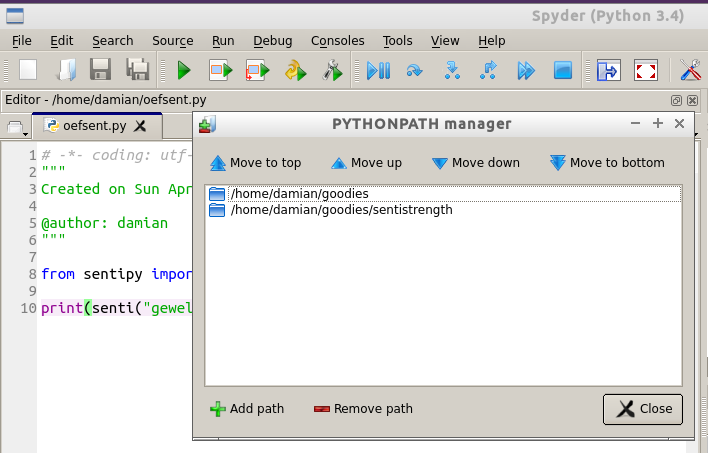
\includegraphics[width=.8\textwidth, keepaspectratio]{../pictures/pythonpath}
	\caption{\label{fig:pythonpath}Telling spyder where to find additional modules}
\end{figure}


Now you can test wether everything works:


\begin{lstlisting}
from sentipy import senti
print(senti("geweldig nieuws","dutch"))
\end{lstlisting}

You see that it returns a list with two values, the first one being the positivity (on a scale from 1 to 5), the second one being the negativity (on a scale from $-1$ to $-5$).

So, let's run it on a real dataset. Why not open a JSON file with some paragraphs from State-of-the-Union speeches (which I exported from AmCAT \citep{VanAtteveldt2008}) and write the text, the positivity score, and the negativity score to a csv file?

You can get the speeches here:
\begin{lstlistingbash}
wget https://raw.githubusercontent.com/damian0604/bdaca/master/examples/stateoftheunion.json
\end{lstlistingbash}

And this is the Python code:

\begin{lstlisting}
from sentipy import senti
import csv
import json
with open("stateoftheunion.json",mode="r",encoding="utf-8") as fi:
       articles=json.load(fi)
with open("articles.csv",mode="w",encoding="utf-8") as fo:
    writer=csv.writer(fo)
    for art in articles:
        s=senti(art["text"],"english")
        print(s)
        writer.writerow([art["medium"],art["date"],art["text"],s[0],s[1]])         
\end{lstlisting}

You will surely see that there is a problem, though: It takes almost a second to call \texttt{senti()}. This is because of the not-so-good implementation in this case (we call an external java program each time we want to get the sentiment). We wouldn't have to care about time, but as we have $>20\,000$ paragraphs to analyze, we can either wait six hours or interrupt with \fbox{CTRL-C}. You might have noticed that this time, we did not first create lists that we combined with \texttt{zip}, but that we write each line immediately to the file. This has two advantages: It saves memory, and if we abort, everything we did until that moment has already been written to the output file.

\begin{question}Can you extend the algorithm in Chapter~\ref{simplesent}, so that additional columns based on the Sentistrength-algorithm are saved? \\ Can you also implement some way of comparing the outcomes of both approaches?
\end{question}

The reason why the above approach is so slow, however, is not the sentiment analysis \emph{itself}, it is the the fact that the external Java program has to be \emph{started} $20\,000$ times. It would be more efficient to do this only once (MUUUUUCH more efficient, in fact). The approach below takes \emph{less than a minute} to run. It saves the $20\,000$ texts to analyze in \emph{one} text file, one per row (thus, all line breaks within each text are removed before) and then tells sentistrength to calculate the sentiment per line. I wrote a function \texttt{sentifile} to achieve this. 
The \texttt{sentifile} takes two or three arguments: the name of an input file, the language, and optionally a boolean value that indicates wether you want the full text to be returned or not. If False (or ommitted), the function returns a list of (positive, negative)-tuples, if True, it returns (postive, negative, text).

The following sample code illustrates its working>

\begin{lstlisting}
from sentipy import sentifile
import csv
import json

with open("stateoftheunion.json",mode="r",encoding="utf-8") as fi:
       articles=json.load(fi)

with open("textonly.txt",mode="w",encoding="utf-8") as fo:
    for art in articles:
        fo.write(art["text"].replace("\n"," ").replace("\r"," ").replace("\t", " ") + "\n")

# without text:
with open("scoresonly.csv",mode="w",encoding="utf-8") as fo:
    writer=csv.writer(fo)
    sents=sentifile("textonly.txt","english")
    for s in sents:
        writer.writerow([s[0],s[1]]) 
 
# with text:      
with open("scoreswithtext.csv",mode="w",encoding="utf-8") as fo:
    writer=csv.writer(fo)
    sents=sentifile("textonly.txt","english",True)
    for s in sents:
        writer.writerow([s[2],s[0],s[1]]) 
\end{lstlisting}


\section{Alternatives}
Let us take a step back and compare the approaches we have seen so far. The first one, the simple dictionary approach, was easy to understand and easy to modify, but not very powerful. The second, Vader, was much more powerful. One disadvantage, however, is that it is only available in English. The third one, Sentistrength, is comparable to Vader, but has as big advantage the support of a number of languages, including Dutch. However, this comes at a price: It is not available for free, making it more difficult to share code with others; and it is written in Java, which requires us to use some tricks to actually use it in Python.

But there are more alternatives. For instance, pattern.nl \citep{DeSmedt2012} is very easy to use, open source, and it supports multiple languages. However, it is only available for Python 2 and not compatible with Python 3.

A last, but increasingly popular method for doing sentiment analysis is using supervised machine learning. How to do that will be discussed in Chapter \ref{chap:ml}.


\section{Recap}
You should have understood the general working of different approaches to sentiment analysis. You should know about their pros and cons. Practically speaking, you should be able to
\begin{itemize}
	\item implement a simple, dictionary-based sentiment analysis tool yourself
	\item integrate a tool like Vader or SentiStrength in your own analyses.
\end{itemize}

\chapter{Automated content analysis}
Automated content analysis covers a wide range of techiques, and not all of them can be covered within this tutorial (for an overview and more background information, see \cite{Boumans2016}). We will start with a first, powerful yet easy deductive approach, in which we basically count how often a pre-defined pattern (a search string, for example) occurs. This technique is known as using \emph{regular expressions}. We will then learn how to take characteristics of human language into account to get closer to the real meaning. The technique we use for this is called \emph{Natural Language Processing (NLP)}.
The other approaches to automated content analysis mentioned by \cite{Boumans2016} are discussed in Chapters \ref{chap:network} and \ref{chap:ml}.


\section{Regular expressions}

A regular expression is a \emph{very} widespread way to describe patterns in strings. You probably know wildcards like {\tt{*}} or operators like {\tt{OR}}, {\tt{AND}} or {\tt{NOT}} that you can use in search strings in a lot of applications. But of course this is rather limited: Maybe you want to say somethhing like ``I want all words starting with a letter or a number (but no special character), then a \@-sign, then again some letters, and after the last dot two or three letters (but not more!) letters. You probably saw that this would be some way of describing an email-adress. 

A universal language to formulate such patterns is \emph{regular expressions}. There are some dialects (but the differences are minimal), and you can use them in many editors (!), in the Terminal, in STATA \ldots and in Python.

In its most simple form, a regular expression is just an ordinary search string:
\begin{lstlisting}
python
\end{lstlisting}
finds (``matches") every occurance of the word ``python''. But we can also indicate that two different characters are allowed:
\begin{lstlisting}
[pP]ython
\end{lstlisting}
matches both ``python'' and ``Python''. Some other useful things:

\begin{itemize}
\item \texttt{.} matches \emph{any} character
\item \texttt{[0-9]} matches a digit
\item \texttt{[a-z]} matches all lowercase letters
\item \texttt{[a-zA-Z]} matches all upper- and lowercase letters
\item \texttt{([tT]witter|[fF]acebook)} matches both Twitter and Facebook and is OK with misspelling them as twitter or facebook.
\end{itemize}

You probably got the idea. You can also specify how often sth has to occur:

The item \emph{before} has to occur
\begin{itemize}
\item \texttt{?} 0 or 1 times
\item \texttt{*} 0 or more times
\item \texttt{+} 1 or more times
\end{itemize}
For example,
\begin{lstlisting}
personali[zs]ed-?communication
\end{lstlisting}
matches 
\begin{lstlisting}
personalizedcommunication
personalized-communication
personalisedcommunication
personalised-communication
\end{lstlisting}


There are actually much more possibilities, so download a regular expression cheat sheet (google or try this one: \url{http://www.cheatography.com/davechild/cheat-sheets/regular-expressions/}) to build your own one. Also the wikipedia page on regular expressions is pretty good. You can also play around at \url{http://www.pyregex.com/}.

So, let's try to use regular expressions in Python. There is a whole module for this (its called \texttt{re}) that provides a lot of interesting functions for finding and replacing stuff based on regular expressions.

\begin{itemize}
\item {\texttt{re.findall("\lbrack Tt\rbrack witter|\lbrack Ff\rbrack acebook",testo)}} returns a list with all occurances of Twitter or Facebook in the string called {\texttt{testo}}
\item {\texttt{re.findall("\lbrack 0-9\rbrack +\lbrack a-zA-Z\rbrack +",testo)}} returns a list with all words that start with one or more numbers followed by one or more letters in the string called {\texttt{testo}}
\item {\texttt{re.sub("\lbrack Tt\rbrack witter|\lbrack Ff\rbrack acebook","a social medium",testo)}} returns a string in which all all occurances of Twitter or Facebook are replaced by "a social medium"
\item \texttt{re.match(" +(\lbrack 0-9\rbrack +) of (\lbrack 0-9\rbrack +) points",line)} returns  \texttt{None} unless it \emph{exactly} matches the string \texttt{line}. If it does, you can access the part between () with the \texttt{.group()} method.
\end{itemize}


The difference between \texttt{findall} and \texttt{match} is thus that  \texttt{findall} does not care about what it finds before and after the pattern, while \texttt{match} requires the whole line to be matched.

An example to illustrate the use:

\begin{lstlisting}
line="             2 of 25 points"
result=re.match(" +([0-9]+) of ([0-9]+) points",line)
if result:
   print ("Your points:",result.group(1))
   print ("Maximum points:",result.group(2))
\end{lstlisting}
would produce the following output:
\begin{lstlistingoutput}
Your points: 2
Maximum points: 25
\end{lstlistingoutput}
This is cool, isn't it? We now know how to extract information from a semi-structured string so that we can store it in variables for further analysis!

On page~\pageref{greedy}, you can find some additional information about some regular expression features, especially about the difference between lazy matching and greedy matching, which basically specifies where to ``stop" when a regular expression contains something like \texttt{.*} (thus, matching an arbitrary number of arbitrary characters, which is in fact much more useful than it sounds).


\begin{question}
Can you write a program (a so-called parser) that takes a semi-structured input file of your choice (maybe something you downloaded somewhere) as input and uses regular expressions to store the data in a structured way in a CSV table?
\end{question}


\section{Natural language processing}
\label{sec:nltk}
To prepare, we have to install some more ressources. Run the following Python lines:


\begin{lstlisting}
import nltk
nltk.download()
\end{lstlisting}
A graphical interface is opened (Figure~\ref{fig:nltkdownload}).

\begin{figure}[h]
\centering
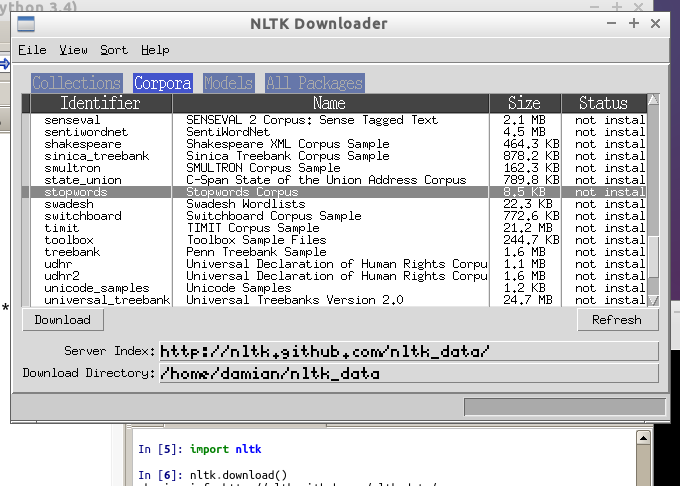
\includegraphics[width=.5\paperwidth,,keepaspectratio]{../pictures/nltk-download.png}
\caption{\label{fig:nltkdownload}Loading additional NLTK-packages}
\end{figure}

Do \emph{not} download all packages, that will take too much space and you do not need it. Instead, download only the packages ``stopwords'' , ``punkt'', and ``maxent\_treebank\_pos\_tagger'' from the ``all packages'' tab. Close the window when done.

\subsection{Stopword removal}

Natural language processing is a term that is used to describe a set of techniques used to analyze language written by humans. This comprises simple tasks like the removal of stopwords in order to identify ``relevant'' words, but also much more complicated things like parsing of a sentence -- which means to automatically identify, for instance, subject, verb and object in a sentence. The book by \cite{Bird2009} gives a comprehensive introduction into NLP with Python. The author also provide the Python package \texttt{nltk}, which we use here.


To find out all the possibilities, have a look at \url{nltk.org}, but here are some examples.

Let us first consider stopword removal. These are words without a meaning that is specific to a text, such as ``a", ``the", \ldots. They are usually more disturbing than useful, because they hinder us from seeing the really interesting words. Keeping them in can lead to misleading results if we want to identify key terms (e.g., by means of a word count), if we want to calculate document similarities, or if we want to make a word co-occurance graphs. A very straightforward way to do so would be the following algorithm, which you -- with the knowledge you gained so far -- actually could have written yourself:

\begin{lstlisting}
t = 'let us clean this up for her'
tn = ""
stopwords=['and','the','this','a','or','he','she','him','her','us']
for w in t.split():
    if w not in stopwords:
       tn=tn+w+" "
\end{lstlisting}

Instead of defining the list in the script itself, we could also read them from a file. Imagine we have a file called \texttt{stopwords.txt} in which we put one stopword per line (we could easily create such a file in \texttt{gedit} or Leafpad or any other text editor):

\begin{lstlistingoutput}
he
she
it
we
they
\end{lstlistingoutput}

We could read this file to a list with

\begin{lstlisting}
stopwords=[w.strip() for w in open("stopwords.txt",encoding="utf-8").readlines()]
\end{lstlisting}

Especially if we have a very long list, this makes our code much easier to read and to maintain. We could also use one of the pre-defined lists provided by \texttt{nltk}, but often, we might want to tweak it to our research interests anyway.

\begin{lstlisting}
from nltk.corpus import stopwords
stopwords=stopwords.words('dutch')
\end{lstlisting}

\subsection{Stemming}
Another interesting step is \emph{stemming}. When interpreting text, we usually do not want to distinguish between smoke, smoked, smoking. Stemming reduces all of these forms to their stem \texttt{smoke}. Therefore, it is a typical preprocessing step (like stopword removal).

So, we could split a given string into words, then stem each word, and combine them again.


\begin{lstlisting}
from nltk.stem.snowball import SnowballStemmer
stemmer=SnowballStemmer("english")
s="I am running while generously greeting my neighbors"
stems=""
for w in s.split():
    stems=stems + stemmer.stem(w)  + " "
\end{lstlisting}

We can now \texttt{print(stems)} to see how the stemmed string looks like.

\begin{quote}
The last three lines can be replaced by a single line: \\
\texttt{stems=" ".join([stemmer.stem(w) for w in s.split()])}
\\
The technique used for it is called \emph{list comprehension} and a really cool feature, google it if you want to know more. In addition, the \texttt{.join()} method allows to join elements from a list to a single string. These two things are considered very pythonic and good coding style, so if you do this kind of stuff more often, it is useful to understand the working (but you can as well use the more elaborate way used in the example). In fact, also the stopword removal could be done in this way: Assuming we have a list with stopwords called \texttt{stopwords} and a sentence \texttt{s} from which we want to remove all stopwords, we can do so with \\
\texttt{s2=" ".join([w for w in s.split() if w not in stopwords])} \\
In doing so, we can create a new string \texttt{s2} with one single line of Python code in which we first split s into a list of words, then make a new list out of these words in which only those words are included that are not in the stopword list, and finally join this list into a single string seperated by spaces.
\end{quote}

\subsection{Part-of-speech tagging}

By parsing sentences, we can find out what grammatical function the words within each sentence has. To this end, NLTK first splits sentences into words (it is called \emph{tokenizing}). But, in addition to what we have done before with the \texttt{.split()} method, it attaches a label to each token that identifies the grammatical characteristics of each token.

\begin{lstlisting}
import nltk
sentence = "At eight o'clock on Thursday morning, Arthur didn't feel very good."
tokens = nltk.word_tokenize(sentence)
print (tokens)
tagged = nltk.pos_tag(tokens)
print(tagged)
\end{lstlisting}

We see that we get a list of tuples (pairs of two values): 
\begin{lstlistingoutput}
[('At', 'IN'), ('eight', 'CD'), ("o'clock", 'JJ'), ('on', 'IN'), ('Thursday', 'NNP'), ('morning', 'NN')]
\end{lstlistingoutput}

This is pretty useful, because we can address the items with \emph{slicing}. For example, to get the fifth tuple, we can write \texttt{tagged[5]}. Of course, we can also slice the tuple. So, to get only the grammatical function of the word ``morning'', we can use  \texttt{tagged[5][1]}. Look up the meaning of the abbreviations like 'NN' up in the documentation. Chapter~5 in \cite{Russel2013} also provides a lot of examples.



\section{Recap}
You should have understood
\begin{itemize}
\item How to remove stopwords
\item How to stem a sentence
\item How to parse a sentence and employ POS tagging
\item How to use NLTK
\end{itemize}




\chapter{Web scraping}
\label{chap:scraping}
\label{parsing}
\section{Overview}
When scraping data from the web, we can distinguish two different stages:
\begin{enumerate}
\item Downloading a (possibly large) number of webpages 
\item Parsing the content of the webpages
\end{enumerate}
Let us start with the first point. Sometimes, we have a list with all URLs of all Dutch news items of the last year, for example, because we retrieved them from a RSS feed. In this case, downloading the data is trivial. We could for exampe use a for-loop in Python, or use the command \texttt{wget} from the bash command line. If we have a file \texttt{urls.txt} that contains one URL per row, we can download all urls with the command
\begin{lstlistingbash}
wget -i urls.txt
\end{lstlistingbash}
We could use a number of additional options, in particular waiting between the URLs to avoid gettig blocked, or pretend that we use a specific web browser. \texttt{wget --help} or Google give you more information.

If we do not have such a list, but rather want to start from one page (e.g., the homepage of a specific website) and simply follow all links that we find on that page, we have to resort to a technique called \emph{crawling}. If we for example want to download the page \url{http://gsc.uva.nl/}, including all links, plus all links encountered on the pages linked to (but stop after this second level of recursion), we can simply type
\begin{lstlistingbash}
wget -l2 http://gsc.uva.nl/
\end{lstlistingbash}
The internet is full of examples (like here: \url{http://www.thegeekstuff.com/2009/09/the-ultimate-wget-download-guide-with-15-awesome-examples/})

At the end of this chapter, I will point you to a framework that allows crawling with Python.

But first, let us turn to the second point: Parsing the content of the pages we downloaded. In virtually all cases, we do not care about the webpage as we downloaded it, but we rather want to extract \emph{some} information in a meaningful way. For example, on a page with product reviews, we want to get rid of all advertisements, navigation elements, \ldots --- in fact, everything except the reviews themselves, which we probably want to store in a list or a similar data structure.

In the next section, we will do so with an approach you are already familiar with: regular expressions. This is useful to show the general idea, and you could use a similar approach a wide range of input data, not only web pages (think of the LexisNexis example). However, especially with complicated HTML pages, this approach can become cumbersome. We will therefore learn how to use XPath descriptions to parse a webpage in another section. 


\section{A simple regular-expression based approach}

First of all, have a look again at the materials about regular expressions. In particular, have another loot at how the \texttt{re.findall()} function can be used to get a list of all strings that match a regular expression within another string. 

Then, open Firefox and go to \url{http://www.geenstijl.nl/mt/archieven/2014/05/das_toch_niet_normaal.html}. Even if you do not understand a word (which actually might help you to look at the structure rather than the content!), you will see that the article is followed by a whole bunch of comments. Already think about a way how one could identify the comments

Click on Tools/Web Developer/Page source (or press \fbox{CTRL-U}) to inspect the source code (Figure~\ref{fig:geenstijlsource}).


\begin{figure}[h]
\centering
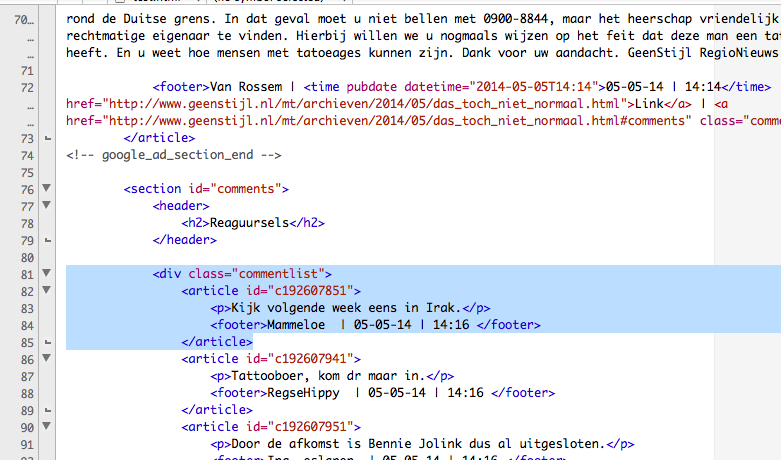
\includegraphics[width=.75\textwidth,keepaspectratio]{../pictures/geenstijl_sourcecode_detail.png}
\caption{\label{fig:geenstijlsource}Examining the source code of a HTML page}
\end{figure}

You should see that the whole block of comments starts with the tag \texttt{<div class="commentlist">} (and, much later, ends with \texttt{</div>}). Also, you should see that each comment starts with a tag \texttt{<article id="xxxxxxxxx">} and ens with \texttt{</article>}.

This looks like a regular pattern, therefore, we can match it with a regular expression. Assuming that the whole page is called \texttt{tekst}, we can get the whole comment section with:
\begin{lstlisting}
commentsection=re.findall(r'<div class="commentlist">.*?</div>',tekst)
\end{lstlisting}
\label{greedy}
Pay attention that we write \texttt{.*?} instead of \texttt{.*} only. The \texttt{.} matches every character, and \texttt{*} means an arbitrary number of times, therefore \texttt{.*} \emph{also} matches \texttt{</div>}. This means that our regular expression would only stop at the \emph{last} occurrence of \texttt{</div>} if there are several ones instead of the \emph{first} one. This is referred to as \emph{greedy matching}. Using \texttt{.*?} instead of \texttt{.*} means that we want to perform \emph{lazy matching} instead, where we do stop as soon as the next part of the regular expression is matched.


As \texttt{re.findall()} returns a list of all matches, \texttt{commentssection} is a list of all commentssections. As there is only one comment section (which we can verify by calculating \texttt{len(commentssection)}, we can get the whole chunk of HTML-code of the comment section by accessing the first and only element of the list, \texttt{commentssection[0]}. 

Now, we can do the same for each comment ("article") within the comment section:

\begin{lstlisting}
comments=re.findall(r'<article.*?>(.*?)</article>',commentsection[0])
\end{lstlisting}

Voilà! We got a list of all comments!

But wait, why did we write the \texttt{()} around\texttt{(.*?)}? This simply means that only the part between \texttt{()} is returned. In other words, \texttt{comments} contains only what is \emph{between} \texttt{<article.*?>} and \texttt{</article>}.

If we now but all this together, add some code to actually download the data (and to also parse the metadata, like author and time of writing), we get the following script:

\begin{lstlisting}
from urllib import request
import re
import csv

onlycommentslist=[]
metalist=[]

req = request.Request('http://www.geenstijl.nl/mt/archieven/2014/05/das_toch_niet_normaal.html', headers={'User-Agent' : "Mozilla/5.0"})
tekst=request.urlopen(req).read()
tekst=tekst.decode(encoding="utf-8",errors="ignore").replace("\n"," ").replace("\t"," ")

commentsection=re.findall(r'<div class="commentlist">.*?</div>',tekst)
print (commentsection)
comments=re.findall(r'<article.*?>(.*?)</article>',commentsection[0])
print (comments)
print ("There are",len(comments),"comments")
for co in comments:
    metalist.append(re.findall(r'<footer>(.*?)</footer>',co))
    onlycommentslist.append(re.findall(r'<p>(.*?)</p>',co))
writer=csv.writer(open("geenstijlcomments.csv",mode="w",encoding="utf-8"))
output=zip(onlycommentslist,metalist)
writer.writerows(output)
\end{lstlisting}


Of course, rather than just saving it to a csv file, we could also add one or two lines to the for-loop and immediately perform a sentiment analysis!

\begin{quote}
What happens exactly in line 8 to 10? In line 8, we form a HTTP-request to specify what we want to download. We could skip this and just specify the URL, but we want to perform a little trick to fool the other side. As they do not like people scraping their content, we have to conceal that we actually do not use a web browser like normal people. Therefore, we let our program just pretend to be Firefox ("Mozilla"). In line 9, we download the web page. However, what we get is just a number of bytes, and Python does not know which byte corresponds to which character. This is why we use the \texttt{.decode()} method in line 10, which changes the sequence of bytes to a string as we know it. Furthermore, we remove all newlines and tabs from the string, because we want one long, uninterrupted string for further processing (especially, we do not want to care about this when designing our regular expressions). 
\end{quote}
Now, you should be ready to write your own parser for some content you are interested in!

\section{XPath-parsing with lxml}
One does not always have  to reinvent the weel, though. It is useful to understand how parsing would work with regular expressions, and it is very likely to come into a situation where this knowledge can be applied. Especially in the case of HTML pages, though, several parsers exist that can make life easier. 

In the example in the last section, we saw that an element in a HTML page can be nested in another element. In other words, a HTML page can be represented as a tree: For example, the page branches into an article, a navigation section, and a comment sections; the latter than branches into several comments. Each element in this tree can be identified by a so-called XPath. You can compare it with the path of a given file (\texttt{/home/damian/week6/slides.pdf}), where the leftmost element is the "highest" level, and where after each \texttt{/}, it indicates to which lower level one has to turn before finally arriving at the file (\texttt{slides.pdf}).  

The good news is that you can look up the XPath of an element with your web browser (the bad news, though, is that on some pages it can be a bit tricky to get it \emph{exactly} right). In Firefox, you have to install a plugin for that. It is called XPath Checker and you can get it by googling it or from \url{https://addons.mozilla.org/nl/firefox/addon/xpath-checker/}. Install it and restart Firefox.

Now, go to a website of your choice, select the part of content that you want to scrape, right-click on it, and select "View XPath". XPath Checker opens (Figure~\ref{fig:xpathchecker}) and suggests an XPath. It also displays the content that would be selected if one used this XPath.

\begin{figure}[h]
\centering
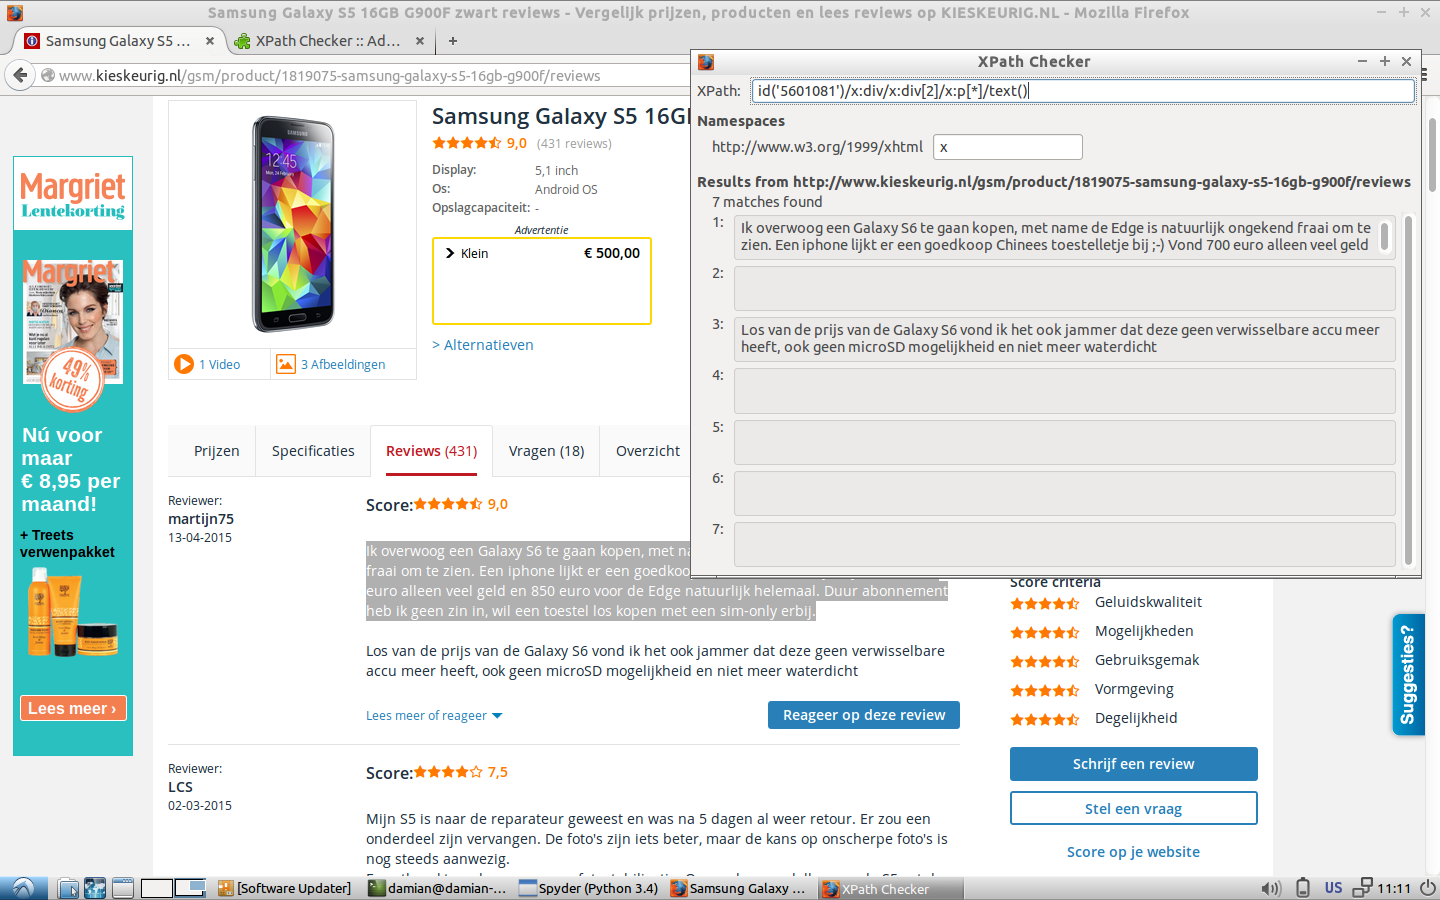
\includegraphics[width=\textwidth,keepaspectratio]{../pictures/xpathchecker}
\caption{\label{fig:xpathchecker}Identifying a correct XPath with XPath Checker}
\end{figure}

Often, you do not only want that \emph{one} comment you selected, but \emph{all} comments. Nevertheless, select just one, and then try to modify the XPath until it fits your needs. The XPath Checker immediately shows you the results, so you can engage in a lot of trial- and error. Some rules for modifying the XPath:

\begin{itemize}
\item \texttt{//} (thus, a double slash rather than a single slash) means `arbitrary depth' (=may be nested in many higher levels, there may be an arbitrary number of higher levels which are not further specified)
\item \texttt{*} means `anything' (if \texttt{p[2]} is the second paragraph, \texttt{p[*]} are all paragraphs)
\item Let the XPath end with \texttt{/text()} to get all text
\end{itemize}

\begin{quote}
	When there is a line or paragraph break within the results of an XPATH, the \texttt{/text()} function might not function properly, as it sees each part as a separate element. This can be fixed by leaving away the \texttt{/text()} in the XPATH itself and instead using the \texttt{.text\_content()} method later on, as this example illustrates:
	\begin{lstlisting}
reviews = tree.xpath('//div/div/div[2]/div[*]/div[2]/p[1]')
i=0
for review in reviews:
	print("Review",i,":",review.text_content())
	i+=1
\end{lstlisting}	
\end{quote}


In addition, you can also have a look at alternative XPath specifications. Again, select the text you are interested in, right-click, and choose ``Inspect element''.\footnote{If you use the Chrome browser, you can directly copy an XPath from the ``Inspect element'' window, but you have no way of interactively checking the XPath like with the Firefox XPath Checker.} You can now see how the HTML tags referring to that element are nested, which should correspond to the construction of your XPath (Figure~\ref{fig:inspectelement}). In particular,
\begin{itemize}
\item If you want to refer to a specific attribute of a HTML tag, you can use \texttt{@}. For example, every \texttt{*[@id="reviews-container"]} in an XPath would grab what is within a tag like \texttt{<div id="reviews-container" class="user-content">}
\end{itemize}


\begin{figure}[h]
	\centering
	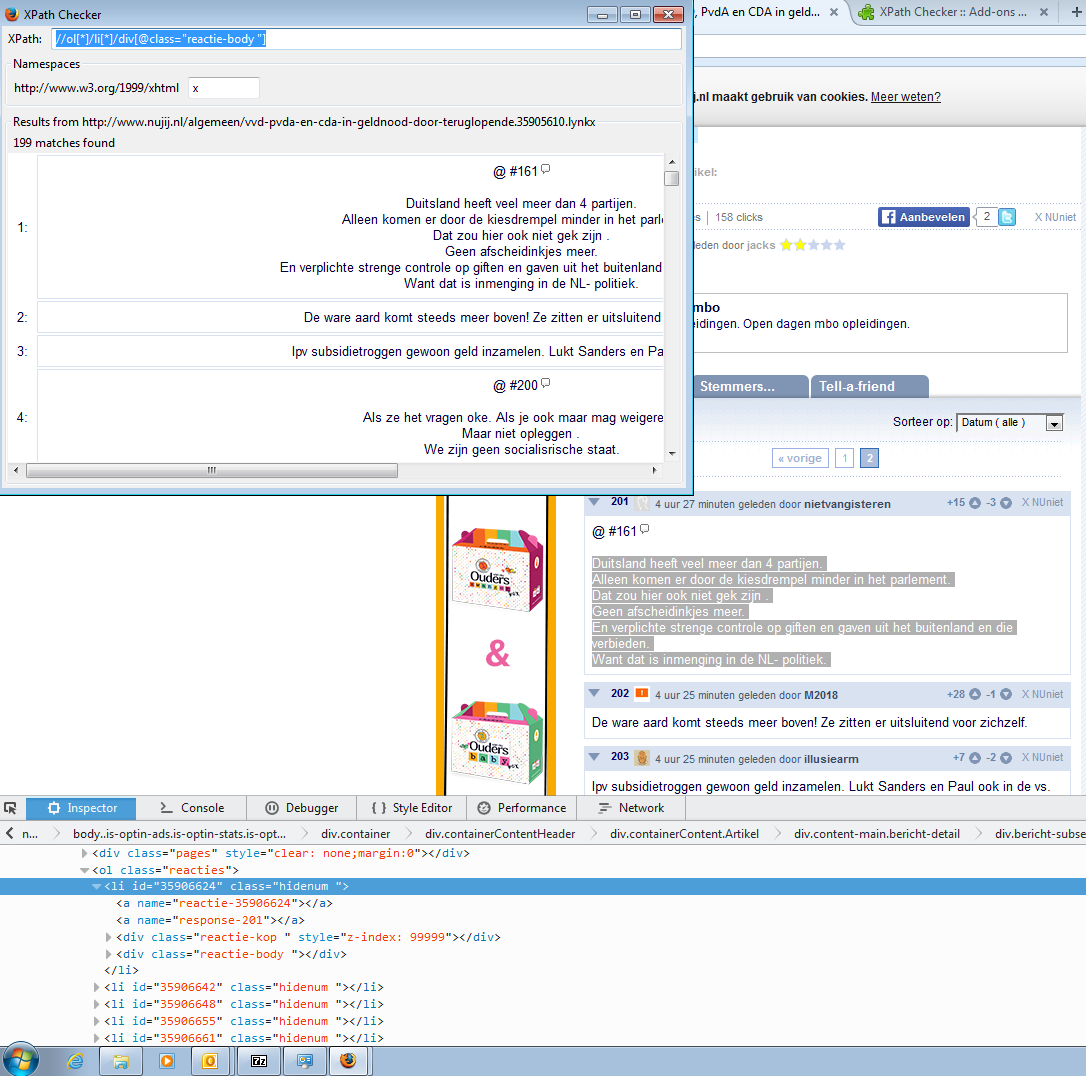
\includegraphics[width=\textwidth,keepaspectratio]{../pictures/inspectelementcrop}
	\caption{\label{fig:inspectelement}Gathering information for constructing an alternative XPATH specification, using the ``inspect element'' function.}
\end{figure}


An example that scrapes all reviews of a specific telephone using one single XPath expression:

\begin{lstlisting}
from lxml import html
from urllib import request

req=request.Request("http://www.kieskeurig.nl/smartphone/product/2334455-apple-iphone-6/reviews")
tree = html.fromstring(request.urlopen(req).read().decode(encoding="utf-8",errors="ignore"))        

reviews = tree.xpath('//*[@class="reviews-single__text"]/text()')

# remove empty reviews and remove leadint/trailing whitespace
reviews = [r.strip() for r in reviews if r.strip()!=""]

print (len(reviews),"reviews scraped. Showing the first 60 characters of each:")
i=0
for review in reviews:
    print("Review",i,":",review[:60])
    i+=1
\end{lstlisting}


This produces the following output:

\begin{lstlistingoutput}
67 reviews scraped. Showing the first 60 characters of each:
Review 0 : De Apple Iphone 6 Zilver/16GB het is een heel fijn apparaat 
Review 1 : Apple maakt mooie toestellen met hard- en software uitsteken
Review 2 : Vanaf de iPhone 4 ben ik erg te spreken over de intuitieve i
Review 3 : Helaas ontbreekt het Apple toestellen aan een noodzakelijk i
\end{lstlistingoutput}

Now it's your turn!


\section{Alternatives}
You can get very far with the approaches sketched in this chapter: regular expressions, the lxml-package, and wget for automated downloading tasks. BeautifulSoup is a python package that lies somewhere in between, as it resembles lxml, but internally uses regular expressions rather than an XPath to parse the HTML. Within lxml, you can also use so-called CSS selectors instead of XPATHs.

If you want to write an application that integrates crawling and parsing, you might have a look at the scrapy framework (\url{http://scrapy.org/}), although it might be a bit of an overkill.

One approach that we haven't covered is how to scrape content from sites that do complicated stuff like interactively loading data while they are visited. For example, think of a news site that uses a JavaScript to display comments: these comments may not be present in the HTML code of the site, but might be dynamically loaded while the user is reading the article. In such a case, one can make use of a framework like Selenium (google "selenium python" or ask your instructor for some examples). Selenium allows you to start a browser, click somewhere, and so on (in essence, it just automates what a human would do), and then parse what is displayed in the browser. 

\section{Recap}
You should be able to write your own web scraper. This entails that you
\begin{itemize}
	\item have a global understanding of how a HTML page looks like, so that you can use this information to build your scraper
	\item understand that there are several ways to parse a specific piece of information from a page
	\item know not only regular expressions, but also how to use packages like lxml.
\end{itemize}


\chapter{Network visualization}
We are often used to representation of data in forms of two-dimensional tables (an Excel or SPSS file, a CSV file). We have already seen that this is not always the most appropriate way to conceptualize data: Hierarchical data, for example, can often be much better represented in JSON format. Another way of representing data is in form of a \emph{network} (Figure~\ref{fig:networkwords}).

\begin{figure}[h]
\centering
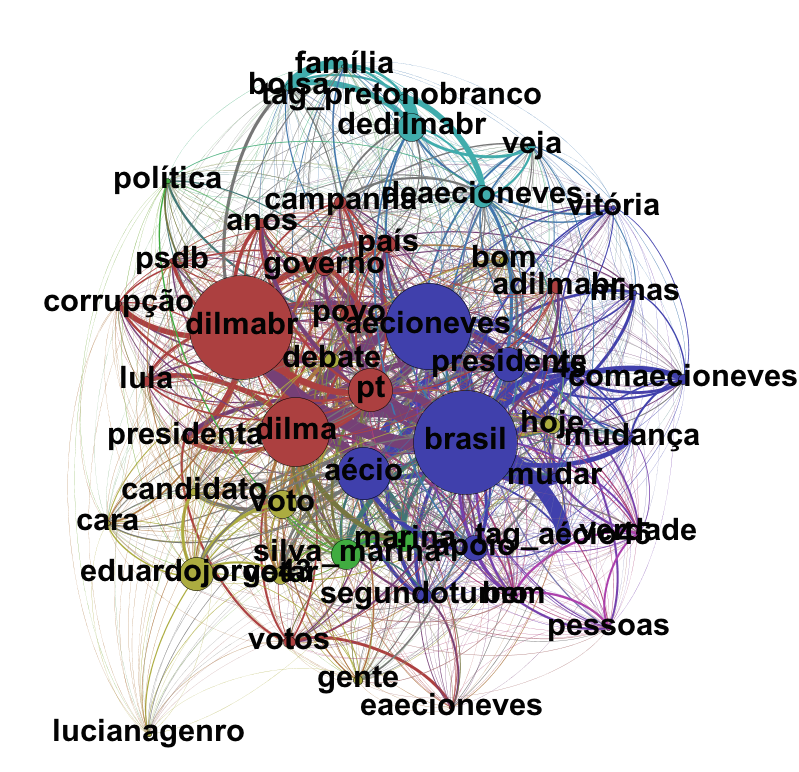
\includegraphics[width=.5\paperwidth,,keepaspectratio]{../pictures/networkwords.png}
\caption{\label{fig:networkwords}A network of co-occuring words}
\end{figure}

We call the elements in a network \emph{nodes} and the connections between them \emph{edges}. A node can be anything: a word, a person, whatever. Edges van be directed (like an arrow) or undirected. For example, a nework of Twitter users (the edges) could have edges that represent \@-mentions. These edges would be directed: if A mentions B, that does not imply that B mentions A as well. On a Facebook friendship network, this would be different: Here, we would have undirected edges.

Giving an introduction to network analysis falls outside of the scope of this tutorial, but you will learn how to save your data in a format that can be used to analyze or visualize them. 

In particular, we will look how we can construct a network of words that co-occur together in texts, which can be a nice way to conduct some inductive framing analysis \citep[see][]{Boumans2016,Trilling2015}.

\label{chap:network}
\section{Producing a file for analysis with Gephi}
Let us considering the following case: We have a list of strings (e.g., a list of tweets) and want to know which words often occur together in the same string (tweet). We could model our data in such a way that each word is a node. We could also attach a weight to each node, so that the node can be displayed bigger the more often the word is mentioned. We could now say that if two words co-occur together, they are connected with a node. Again, we could say that the more often this happens, the thicker the edge should become.

Thus, we basically need 
\begin{itemize}
\item a list with all words (the nodes) with their frequency (the weight/size of the nodes)
\item a list with all connections (the edges, thus, a list of pairs of nodes that are co-occuring in the same string/tweet) with the number of strings/tweets in which they co-occur.
\end{itemize}
The GDF file format is a format that allows us to store exactly this information. Have a look at the following example. In lines 1, it is defined how the following node definitions are formated: a variable called \texttt{name}, which is a string (that's what they mean with VARCHAR), followed by a variable \texttt{width} which has the format double (a type of number, we would call it a float). And indeed, you see that the following lines contain strings (the words which are the nodes) followed by the size of the node (the frequency of the words).
In line 12, it is defined that the following lines contain the edge definitions: two strings (node1 and node 2, followed by the edge weight.

For example, we see that the words ``coffee'' occurs three times in total (line 2), and one time together with the word ``beer'' (line 13).


\begin{lstlistingoutput}
nodedef>name VARCHAR, width DOUBLE
coffee,3
beer,2
i,4
and,1
with,1
friend,1
having,1
like,3
am,1
my,1
edgedef>node1 VARCHAR,node2 VARCHAR, weight DOUBLE
coffee,beer,1
i,beer,2
and,beer,1
with,friend,1
coffee,with,1
i,and,1
having,friend,1
like,beer,2
am,friend,1
i,am,1
i,coffee,3
i,with,1
am,having,1
i,having,1
coffee,and,1
like,coffee,2
am,coffee,1
with,my,1
i,friend,1
like,and,1
am,with,1
having,with,1
i,my,1
having,coffee,1
i,like,3
coffee,friend,1
having,my,1
am,my,1
coffee,my,1
my,friend,1
\end{lstlistingoutput}

As the format is so simple, we can write a program that produces such a file. In fact, we have already done so for the first part: it is in fact nothing else than a CSV file with frequency counts. 

For the second part, we need a module that tells us wich words co-occur together. In other words, we want to know all \emph{combinations} of words in a given string. Not very surprisingly, this method is called \texttt{combinations}. See the example below:

\begin{lstlisting}
from itertools import combinations
words="Let's combine stuff!".split()
print ([e for e in combinations(words,2)])
\end{lstlisting}
produces:

\begin{lstlistingoutput}
[("Let's", 'combine'), ("Let's", 'stuff!'), ('combine', 'stuff!')]
\end{lstlistingoutput}

We already see that it is probably wise to do some preprocessing (to remove the punctuation for example, but you can also think of stopword removal, stemming, or converting to lowercase. We will leave that for know, you already know how to do this and can add that yourself.

There is one thing we still have to consider: We have an undirected network and do not want to distinguish between \texttt{('combine', 'stuff!')} and \texttt{('stuff!', 'combine')}. We can construct the following minimal example, where we print a list of edges, based on co-occurrances of words in a set of three tweets. Do you see how we use lines 8 and 9 to turn around \texttt{('stuff!', 'combine')} if we already have  \texttt{('combine', 'stuff!')} in our dict of edges that we construct? Also look at line 10, where we specify that a combination is only added to the dict (in line 11) if both nodes are not identical.

\begin{lstlisting}
from collections import defaultdict
from itertools import combinations
tweets=["i am having coffee with my friend","i like coffee","i like coffee and beer","beer i like"]
cooc=defaultdict(int)
for tweet in tweets:
    words=tweet.split()
    for a,b in set(combinations(words,2)):
        if (b,a) in cooc:
            a,b = b,a
        if a!=b:
            cooc[(a,b)]+=1
for combi in sorted(cooc,key=cooc.get,reverse=True):
    print (cooc[combi],"\t",combi)
\end{lstlisting}

This gives you:

\begin{lstlisting}
3 	 ('i', 'coffee')
3 	 ('i', 'like')
2 	 ('like', 'coffee')
2 	 ('i', 'beer')
2 	 ('like', 'beer')
1 	 ('i', 'am')
1 	 ('am', 'friend')
\end{lstlisting}

You know have all building blocks you need to write a program that produces a GDF file. You would need to add
\begin{itemize}
\item something that reads your input from a file (e.g., a CSV file of tweets or a JSON file of speeches or a set of individual TXT files with newspaper articles)
\item some preprocessing
\item maybe some filter to filter out nodes and edges that occur very few times
\item something to write the output to a file rather than printing to the screen.
\end{itemize}

The GDF file your program produces can be opened in Gephi (or some other network visualization or analysis tool). I made a screencast where I quickly show how to use Gephi. You can watch it here: \url{https://streamingmedia.uva.nl/asset/detail/t2KWKVZtQWZIe2Cj8qXcW5KF}.
\begin{quote}
Rather than producing a GDF file and opening it in Gephi, you can also do network analysis in Python itself, for example with the module \texttt{networkx}. This can be very interesting, especially for really large networks (which you maybe cannot open with a graphical tool like Gephi).
\end{quote}



\section{Recap}
This chapter taught you how to deal with co-occurrences and similar structures from a network point of view and how to visualize them using Gephi. More in general, you also should have seen how one can write own programs to create specific file formats, even if they are not natively supported.




\chapter{Machine learning and topic modelling}
\label{chap:ml}
The vastness of the topic makes it impossible to cover it extensively in this course. Nevertheless, as last part, we will take a very small and superficial glimpse in the world of supervised and unsupervised machine learning. The lecture slides should give you a bit more context, but here you find two examples to illustrate the general principle --- and to give you a starting point for your own investigations. We will use scikit-learn \citep{scikit-learn} and gensim \citep{Rehurek2010}, two packages that are very widely used and for which you will find a lot of tutorials and usage examples on the web.

\section{Supervised machine learning}
For this demonstration, we use a dataset from the Internet Movie Database \citep{Maas2011}. It contains in total $50 000$ reviews, separated into a test dataset and a training datasset ($25 000$ each), half of them positive, half of them negative.

Download and unpack the dataset:

\begin{lstlistingbash}
cd /home/damian
wget http://ai.stanford.edu/~amaas/data/sentiment/aclImdb_v1.tar.gz
tar -xzf aclImdb_v1.tar.gz
rm aclImdb_v1.tar.gz
\end{lstlistingbash}

You now have a folder \texttt{aclImdb} in your home directory. Take a look at the structure of the dataset, maybe read the documentation that is included.

You should probably see rather quickly that there are two folders with an identical structure, \texttt{train} and \texttt{test}. Within each of them, there are two folders \texttt{pos} and \texttt{neg}, with a lot of plain text files within them. Have a look at them. 

First of all, we need the training dataset and the test dataset. Lets conceptualize them as a list of tuples	where all positive reviews get a 1, and all negative ones a $-1$:

\begin{lstlisting}
reviews=[("This is a great movie",1),("Bad movie",-1), ... ...]
test=[("Not that good",-1),("Nice film",1), ... ...]
\end{lstlisting}

Of course, we do not want to insert our $50 000$ reviews by hand, but read them from the files we downloaded. We did something similar already with for example the LexisNexis articles or the lists of positive or negative words. Let's do it using the package \texttt{glob} that makes our live easier here:

\begin{lstlisting}
from glob import glob

reviews=[]

for file in glob ("/home/damian/aclImdb/train/pos/*.txt"):
    with open(file) as fi:
        reviews.append((fi.read(),1))

for file in glob ("/home/damian/aclImdb/train/neg/*.txt"):
    with open(file) as fi:
        reviews.append((fi.read(),-1))
\end{lstlisting}


After that, we do exactly the same for the test dataset. You only have to replace \texttt{reviews} with \texttt{test} in the code above, and \texttt{train} with \texttt{test}.

Once we have done this, and thus have two lists, \texttt{reviews} and \texttt{test}, each of them with a length of $25 000$, we can train and test the classifier --- after importing the necessary modules from the package scikit-learn \citep{scikit-learn}, of course:

\begin{lstlisting}
from sklearn.naive_bayes import MultinomialNB
from sklearn.feature_extraction.text import CountVectorizer
from sklearn import metrics
\end{lstlisting}

We use a Bag-of-Word representation of all reviews rather than the whole reviews. We only want to know the frequency of each word in each review. While we could calculate this ourselves, scikit-learn integrates this nicely in the workflow (they even remove stopwords for us):

\begin{lstlisting}
vectorizer = CountVectorizer(stop_words='english')
train_features = vectorizer.fit_transform([r[0] for r in reviews])
test_features = vectorizer.transform([r[0] for r in test])
\end{lstlisting}

\begin{quote}
Note that \texttt{[r[0] for r in reviews]} is a short form of writing something like the following (it is called ``list comprehension''):
\begin{verbatim}
newlist=[]
for r in reviews:
    newlist.append[r[0]]
\end{verbatim}
It gives us a list of the reviews themselves, without the scores -- and \texttt{r[1]} would give us only the scores.
\end{quote}

Training the machine learning algorithm (we chose the Multinomial Naïve Bayes variant here, there are others as well -- read the docs and check out which one is best!) takes only two lines:
	
\begin{lstlisting}
# Fit a naive bayes model to the training data.
nb = MultinomialNB()
nb.fit(train_features, [r[1] for r in reviews])
\end{lstlisting}

Let's now use the classifier we just trained to predict the classification of our test dataset:

\begin{lstlisting}
predictions = nb.predict(test_features)
actual=[r[1] for r in test]
\end{lstlisting}
(of course, we already know the actual, real classes, we just put them in a list in the second line for easier comparison)

We could compare the two lists \texttt{predictions} and \texttt{actual} by hand to find out in where our classifier is right or wrong. But we can also just calculate the AUC, a measure of accuracy:

\begin{lstlisting}
print(metrics.accuracy_score(actual,predictions,normalize=True))
\end{lstlisting}

We can now play around and see how the classifier classifiers some new data:




\begin{lstlisting}
newreviews=["What a crappy movie! It sucks!",
          "This is awsome. I liked this movie a lot, fantastic actors",
          "I would not recomment it to anyone.",
          "Enjoyed it a lot"]

new_features=vectorizer.transform(newreviews)
predictions = nb.predict(new_features)
print(predictions)

\end{lstlisting}



\subsection{Comparing different classifiers and vectorizers}
Usually, when we de supervised machine larning, we want to compare different classifiers. For example, in the last section, we used a Naïve Bayes classifier. But we could use a logistic regression as well, or a so-called support vector machine. It is common to run several of these models and then compare their \emph{precision} and \emph{recall}. 

Let us assume that the goal of training above-mentioned classifier is to build an app that shows the user only films we can expect to receive positive ratings. There are two things that we want to achieve: We want to find as many as possible positive films (recall), but we also want that the selection we found \emph{only} contains positive films (precision).

Precision is calculated as $\frac{TP}{TP+FP}$, where TP are true postivies and FP are false positives. For example, if our classifier retrieves 200 articles that it classifies as positive films, but only 150 of them indeed are positive films, then the precision is $\frac{150}{150+50} = \frac{150}{200} = 0.75$.

Recall is calculated as $\frac{TP}{TP+FN}$, where TP are true postivies and FN are false negatives. If we know that the classifier from the previous paragraph missed 20 positive films, then the recall is $\frac{150}{150+20} = \frac{150}{170}= 0.88$.

In other words: Recall measures how many of the cases we wanted to find we actually found. Precision measures how much of what we have found actually is correct.

Often, we have to make a trade-off between precision and recall. For example, just retrieving \emph{every} film would give us a recall of 1.0 (after all, we didn't miss a single positive film). But on the other hand, we retrieved all the negative films as well, so precision will be extremely low. It can depend on the task at hand whether precision or recall is more important.

Another thing we can vary in our classifier is the vectorizer we used. In our example, we used a count vectorizer, which simply means that our \emph{features} (which is just a fancy word for independent variables) are simply the frequency counts of the words. This approach has the disadvantage that some words will be very frequent in almost all articles, while others occur in only a few articles. Arguably, such words are more informative and therefore, their occurrence should weigh more heavily. The tf$\cdot$idf scheme does exactly that: it weighs the term frequency (TF) by the inverse document frequency (IDF), i.e. the number of texts (``documents'') in which the word (``term'') occurs at least once.

Scikit-learn allows us to use tf$\cdot$idf scores instead of simple counts by using another vectorizer\footnote{For details, see \url{http://scikit-learn.org/stable/modules/generated/sklearn.feature_extraction.text.TfidfVectorizer.html}}:

\begin{lstlisting}
from sklearn.feature_extraction.text import CountVectorizer, TfidfVectorizer
# instead of:
myfirstvectorizer=CountVectorizer(stop_words='english')
# we could do:
mysecondvectorizer=TfidfVectorizer(stop_words='english')
\end{lstlisting}

Below, you find an example script that combines everything that we discussed in these sections. There are more elegant ways of doing this, for example by writing functions instead of repeating the code that calculates the evaluations, but for illustration purposes, I decided to leave it as it is:




\begin{lstlisting}
#!/usr/bin/env python3
# -*- coding: utf-8 -*-
from glob import glob
from sklearn.naive_bayes import MultinomialNB
from sklearn.feature_extraction.text import CountVectorizer
from sklearn import metrics

reviews=[]
test=[]

print("Constructing training dataset")

# glob gives you a list of filenames that match a specific criterion
# in this case, all .txt-files in the postivie training folder

for file in glob ("/home/damian/aclImdb/train/pos/*.txt"):
    with open(file) as fi:
        reviews.append((fi.read(),1))
nopostr=len(reviews)

print ("Added",nopostr,"positive reviews")  

for file in glob ("/home/damian/aclImdb/train/neg/*.txt"):
    with open(file) as fi:
        reviews.append((fi.read(),-1))
nonegtr=len(reviews)-nopostr
print ("Added",nonegtr,"negative reviews")  
   
print("Constructing test dataset")

for file in glob ("/home/damian/aclImdb/test/pos/*.txt"):
    with open(file) as fi:
        test.append((fi.read(),1))
noposte=len(test)
print ("Added",noposte,"positive reviews")  

for file in glob ("/home/damian/aclImdb/test/neg/*.txt"):
    with open(file) as fi:
        test.append((fi.read(),-1))
nonegte=len(test)-noposte
print ("Added",nonegte,"negative reviews")  

#%% Checking the data
# Thus, we got two lists, reviews and test.
# Both contain tuples (pairs of two values: The first is the review, 
# the second the classification: 1 or -1)
    
# We can easiliy verify this by looking at a random entry:
print(reviews[244])
# or
print('The following review\n\n\n',reviews[244][0],"\n\n\nis evaluated as",reviews[244][1])
    
#%% Training the classifier                

print("Training classifier...")        

# Generate BOW representation of word counts
vectorizer = CountVectorizer(stop_words='english')   
#alternatively, you could provide a list of stop words yourself
train_features = vectorizer.fit_transform([r[0] for r in reviews])
test_features = vectorizer.transform([r[0] for r in test])

# Fit a naive bayes model to the training data.
nb = MultinomialNB()
nb.fit(train_features, [r[1] for r in reviews])

#%% testing the classifier
# Now we can use the model to predict classifications for our test features.
predictions = nb.predict(test_features)
# and also put the 'true' results from the test dataset in a list
actual=[r[1] for r in test]

# now we can compare whether the predicted values and the actual values match.
# We could write the output to a tab seperated file to see what matches:
with open("/home/damian/agreement.tab", mode='w') as fo:
    fo.write("actual\tpredicted\tfirst words\n")
    for i in range(len(predictions)):
        fo.write(str(actual[i])+"\t"+str(predictions[i])+"\t"+test[i][0][:50]+"\n")

# That can be helpful for inspecting where sth goes wrong, but we can  
# also calculate some measures of performance immediately:

print('Accuracy:')
print(metrics.accuracy_score(actual,predictions,normalize=True))

print('Precision:')
print(metrics.precision_score(actual,predictions,pos_label='1', labels = ['-1','1']))
print('Recall:')
print(metrics.recall_score(actual,predictions,pos_label='1', labels = ['-1','1']))

# Note that Precision is not a symmetric measure.
# If we want the precision for retrieving a NEGATIVE review # instead of a positive we get a different value:

print('\t side note: Precision if we are interested in retrieving negative reviews:')
print('\t',metrics.precision_score(actual,predictions,pos_label='-1', labels = ['-1','1']))
print('\t side note: Recall if we are interested in retrieving negative reviews:')
print('\t',metrics.recall_score(actual,predictions,pos_label='-1', labels = ['-1','1']))

# back to normal

print('F1-score:')
print(metrics.f1_score(actual,predictions,pos_label='1', labels = ['-1','1']))
print('Confusion matrix:')
print(metrics.confusion_matrix(actual,predictions))


#%% Now, let's play around and see how well it would work on 
# new unseen data:
newreviews=["What a crappy movie! It sucks!",
            "This is awsome. I liked this movie a lot, fantastic actors",
            "I would not recomment it to anyone.",
            "Enjoyed it a lot"]
newdata=vectorizer.transform(newreviews)
predictions = nb.predict(newdata)
print(predictions)
for i in range(len(predictions)):
    if predictions[i]==1:
        print(newreviews[i],'\nis probably about a GOOD movie\n')
    elif predictions[i]==-1:
        print(newreviews[i],'\nis probably about a BAD movie\n')

\end{lstlisting}


We used a Na\"ive Bayes classifier, but we could as well use a different one, for example a logistic regression\footnote{You can find one explanation of the difference here: \url{https://www.quora.com/What-is-the-difference-between-logistic-regression-and-Naive-Bayes?share=1}. Basically, in contrast to a logistic regression, in a Na\"ive Bayes classifier, all features are assumed to be uncorrelated.}

You can run a logistic regression classifier just as you would run a NB classifier\footnote{We could get more info, see \url{http://scikit-learn.org/stable/modules/generated/sklearn.linear\_model.LogisticRegression.html}. For example, if you are interested in coefficients: \\
	\texttt{predictionsproba = logreg.predict\_proba(test\_features)}\\
	\texttt{print([j for i in logreg.coef\_ for j in i])}}:

\begin{lstlisting}
from sklearn.linear_model import LogisticRegression
logreg = LogisticRegression()
logreg.fit(train_features, [r[1] for r in reviews])
predictions = logreg.predict(test_features)
\end{lstlisting}

A last one would be a support vector macine (SVM) (for more info, see \url{http://scikit-learn.org/stable/modules/svm.html})

\begin{lstlisting}
from sklearn import svm
mysvm = svm.SVC()
mysvm.fit(train_features, [r[1] for r in reviews])
predictions = mysvm.predict(test_features)
\end{lstlisting}

Note that the names I assigned to each classifier (\texttt{nb}, \texttt{logreg}, \texttt{mysvm}) are completely arbitrary.



\subsection{Saving the trained model}

In theory, you could just train the model everytime you want to use it. However, that does not only take unnecessary time and ressources, but it also requires you to have the training data at hand. Therefore, it can be useful to save your vectorizers and classifiers. It is important to realize that you need to save both: After all, the vectorizer determines which word is mapped to which internal numeric representation, that is used by the classifier. 

Once you have fitted both vectorizer and classifier, you can save them as follows (assuming you have called your instance of the vectorizer \texttt{vectorizer} and your instance of the classifier \texttt{nb}):

\begin{lstlisting}
import pickle
from sklearn.externals import joblib

pickle.dump(vectorizer,open("myvectorizer.pkl",mode='wb'))
joblib.dump(logreg, 'myclassifier.pkl')
\end{lstlisting}


Then, later on, instead of fitting a new vectorizer, you can simply load the old one and use it


\begin{lstlisting}
import pickle
vectorizer = pickle.load(open("myvectorizer.pkl",mode='rb'))
new_features = vectorizer.transform([listwithnewdata])
\end{lstlisting}

As you see, you do not do any \texttt{.fit\_transform} any more, because the vectorizer is already fitted (that was why we saved it, after all).

Also the classifier can be loaded again very easily and be used immediately for prediction

\begin{lstlisting}
from sklearn.externals import joblib
nb = joblib.load('myclassifier.pkl')
predictions = nb.predict(new_features)
\end{lstlisting}





\section{Latent Dirichlet Allocation (LDA)}
In the previous chapter, we were had \emph{labeled} data, i.e. we had an outcome which we could predict. In other words, we applied supervised machine learning. But sometimes, we do not have an outcome to predict.For instance, we want to group the films into topics, but we have no idea which topics exist to begin with. 

Topic Modelling therefore is a form of \emph{unsupervised} machine learning. To get to know it, we will use the gensim package \citep{Rehurek2010}. 
	
Furthermore, let us assume you have a list of lists of words (!) called \texttt{texts}:

\begin{lstlisting}
articles=['The tax deficit is higher than expected. This said xxx ...', 'Germany won the World Cup. After a']
texts=[art.split() for art in articles]
\end{lstlisting}
which looks like this:
\begin{lstlistingoutput}
[['The', 'tax', 'deficit', 'is', 'higher', 'than', 'expected.', 'This', 'said', 'xxx', '...'], ['Germany', 'won', 'the', 'World', 'Cup.', 'After', 'a']]
\end{lstlistingoutput}


I'll take the movie reviews from the last section as a test case (without the ratings, which are irrelevant now), but of course you can use any collection of text files.


\begin{lstlisting}
from glob import glob
texts=[]
for file in glob ("/home/damian/aclImdb/train/pos/*.txt"):
    with open(file) as fi:
        texts.append(fi.read().split())
\end{lstlisting}
Pay attention to the \texttt{.split()} method, which makes that we now have a list of lists of words, just as we wanted.

We now let gensim create a BOW representation of the texts --- just as in earlier examples, but each packages has a slightly different syntax for that. Luckily, you don't have to remember that, that's where the documentation and example scripts that come with each package are for.

\begin{lstlisting}
from gensim import corpora, models
# Create a BOW represenation of the texts
id2word = corpora.Dictionary(texts)
mm =[id2word.doc2bow(text) for text in texts]
\end{lstlisting}

We can now train the LDA models:
\begin{lstlisting}
lda = models.ldamodel.LdaModel(corpus=mm, id2word=id2word, num_topics=100, alpha="auto")
\end{lstlisting}

Of course, you can specify any other number of topics. Most people use something like 50 or 100 topics, though. Let's print the most characteristic words for each topic:

\begin{lstlisting}
for top in lda.print_topics(num_topics=NTOPICS, num_words=5):
    print ("\n",top)

\end{lstlisting}

Only one thing left to do: Calculate the scores for each topic per document and save them to a file. I chose a tab-separated one:

\begin{lstlisting}
scoresperdoc=lda.inference(mm)
with open("topicscores.tsv","w",encoding="utf-8") as fo:
    for row in scoresperdoc[0]:
        fo.write("\t".join(["{:0.3f}".format(score) for score in row]))
        fo.write("\n")
\end{lstlisting}

This is the general principle, but of course, there are a lot of ways of tuning it. To start with, some stopword removal would be advisable - and we did not even remove punctuation or all the weird HTML tags, or bother about converting it to lower case. However, you already learned all this and should be able to write a good script by integrating the structure from above with other techniques.

For some suggestions, see the documentation of gensim.% and also the example script I send you.

One particular thing you might want to try, though: Just as in the case of supervised machine learning, also for unsupervised machine learning, you might want to try to use a tf$\cdot$idf vectorizer instead of the default count vectorize. In gensim, you can do so by slightly modifying the script presented above:


\begin{lstlisting}
from gensim import corpora, models
# Create a BOW represenation of the texts
id2word = corpora.Dictionary(texts)
mm =[id2word.doc2bow(text) for text in texts]

# create a tf-idf representation
tfidf = models.TfidfModel(mm)

# use that tfidf-representation instead of the pure counts
lda = models.ldamodel.LdaModel(corpus=tfidf[mm], id2word=id2word, num_topics=100, alpha="auto")
\end{lstlisting}



\section{Recap}
You should be able to explain what supervised and unsupervised machine learning are and give some examples. More practically, you should be able to use the following widely used packages to conduct such analysis:
\begin{itemize}
	\item scikit-learn
	\item gensim
\end{itemize}
In particular, you should be able to not only train models and apply them to new, unseen data, but you should also know how to do a basic evaluation of the performance of the model.



\chapter{Statistics with Python}
\label{chap:statistics}
One of the things you have learned so far is how to output data in a format that suits your needs. For example, no matter what your input data are, you can always save the results of your program in a CSV file that you can open with R, Stata or SPSS for further analysis. And indeed, it can make sense to use different tools in different stages of a project.

However, if you only want to calculate a mean and a standard deviation or even conduct a regression, this is actually not neccessary -- and, let's face it, is pretty cool if your program just does \emph{everything} in a single run. In addition, Python is actually pretty good in doing statistics and used by many data scientists for this purpose. In this chapter, I'll briefly mention some modules that are useful for this, so that you know where to look further.


\section{numpy \& scipy}
Numpy \citep{numpy} is a package that provides a lot of mathematical functions. It can, for example, be used to calculate means (ok, that's boring, you could do that yourself), standard deviations, correlations, and much, much more. It also offers some specific data types that are more efficient for some calculations than the build-in lists. It goes a long with the similar package SciPy \citep{scipy}.



\begin{lstlisting}
import numpy as np
>>> x = [1,2,3,4,3,2]
>>> y = [2,2,4,3,4,2]
>>> np.mean(x)
2.5
>>> np.std(x)
0.9574271077563381
>>> np.corrcoef(x,y)
array([[ 1.        ,  0.67883359],
       [ 0.67883359,  1.        ]])

>>> from scipy import stats
>>> stats.skew(x)
0.0
>>> stats.kurtosis(x)
-0.942148760330578
\end{lstlisting}




\section{matplotlib}


\begin{figure}[h]
\centering
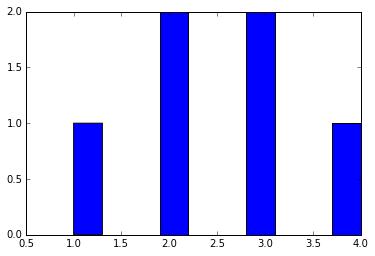
\includegraphics[width=.3\linewidth]{../pictures/plthist}\hfill
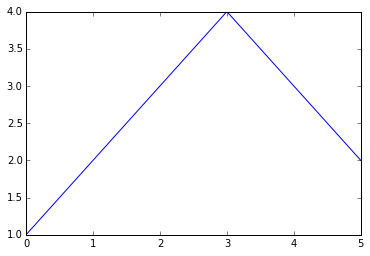
\includegraphics[width=.3\linewidth]{../pictures/pltplot}\hfill
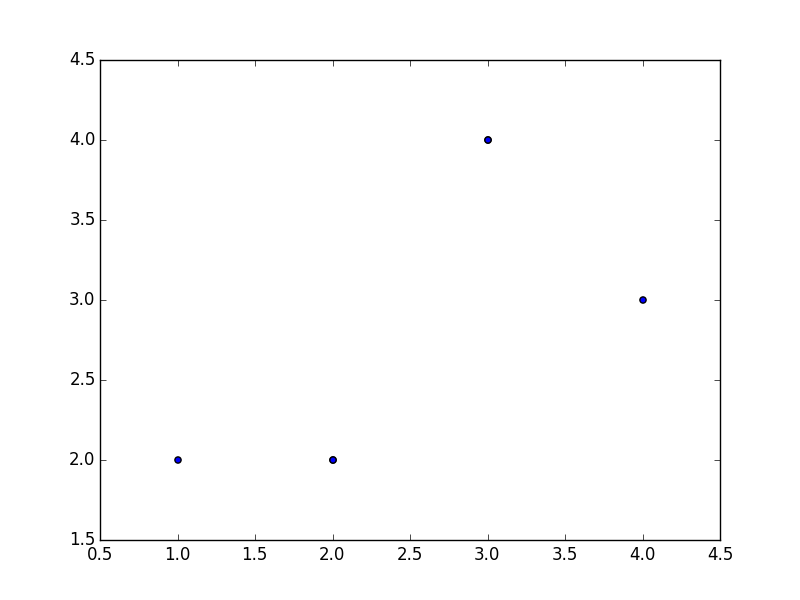
\includegraphics[width=.3\linewidth]{../pictures/pltscatter}
\caption{\label{fig:matplotlib}Examples of plots generated with \texttt{matplotlib}}
\end{figure}


While there are tools that make fancier graphics (take a look at the Python module \texttt{seaborn}; or use \texttt{ggplot2} in R), \texttt{matplotlib} \citep{matplotlib} is really useful if you just want to make a quick histogram, line graph, or scatter plot (Fig.~\ref{fig:matplotlib}).

\begin{lstlisting}
import matplotlib.pyplot as plt
x = [1,2,3,4,3,2]
y = [2,2,4,3,4,2]
plt.hist(x)
plt.plot(x,y)
plt.scatter(x,y)
\end{lstlisting}


\section{pandas \& statsmodels}
Pandas \citep{pandas} is a framework that allows statistical modelling in Python. Those of you who know R will see a lot of similarities. Within pandas, data are stored in a table, very much like a Stata or SPSS dataset -- and yes, it is indeed called exactly as it is called in R: a \emph{dataframe}.
As you see below, a dataframe basically consists of different columns with a name, which consist of a list of data. Pandas can read directly from a CSV file, but as you can see below, you can also construct a dataframe yourself. 

While pandas has a lot of nice functions to explore and manage datasets, it is -- for our purposes -- especially powerful when combined with statsmodels \citep{statsmodels}. Statsmodels allows provides a wide range of models, just like what you would expect from SPSS, Stata, or R.

To run an OLS regression, for example, you only have to specify which columns are the dependent and the independent variables. 

\begin{lstlisting}
import pandas as pd
from statsmodels.formula.api import ols
df = pd.DataFrame({"income": [10,20,30,40,50], "age": [20, 30, 10, 40, 50], "facebooklikes": [32, 234, 23, 23, 42523]}
# alternative: read from CSV file:
# df = pd.read_csv('mydata.csv')

myfittedregression = ols(formula='income ~ age + facebooklikes', data=df).fit()
print(myfittedregression.summary())

\end{lstlisting}
prints a regression table like you would expect from any statistics program:

\begin{lstlistingoutput}
OLS Regression Results                            
==========================================================================
Dep. Variable:                 income   R-squared:                       0.579
Model:                            OLS   Adj. R-squared:                  0.158
Method:                 Least Squares   F-statistic:                     1.375
Date:                Mon, 31 Oct 2016   Prob (F-statistic):              0.421
Time:                        18:11:40   Log-Likelihood:                -18.178
No. Observations:                   5   AIC:                             42.36
Df Residuals:                       2   BIC:                             41.19
Df Model:                           2                                         
Covariance Type:            nonrobust                                         
==========================================================================
coef    std err          t      P>|t|      [95.0% Conf. Int.]
--------------------------------------------------------------------------
Intercept        14.9525     17.764      0.842      0.489       -61.481    91.386
age               0.4012      0.650      0.617      0.600        -2.394     3.197
facebooklikes     0.0004      0.001      0.650      0.583        -0.002     0.003
==========================================================================
Omnibus:                          nan   Durbin-Watson:                   1.061
Prob(Omnibus):                    nan   Jarque-Bera (JB):                0.498
Skew:                          -0.123   Prob(JB):                        0.780
Kurtosis:                       1.474   Cond. No.                     5.21e+04
==========================================================================
\end{lstlistingoutput}

Pandas is a \emph{huge} framework, especially in combination with Jupyter Notebook (Section~\ref{sec:jupyter}). It is extremely popular in the world of data science, but also in areas like finance. 

However, it would be kind of useless to cover it extensively in this intro, as others have already done so. You can have a look at the books by \cite{McKinney2012} and  \cite{Russel2013}. 

You can also find some iPython notebooks with typical analyses with pandas, ranging from correlations and t-tests to regression models and time-series analysis, here: \url{https://github.com/damian0604/bdaca}. 



\section{Recap}
Things you should remember:
\begin{itemize}
	\item There are multiple packages for doing statistical analysis like you know them from programs like SPSS, Stata, or R.
	\item pandas offers you R-like data structures.
	\item There are online ressources with a lot of examples.
\end{itemize}
In particular, once you arrived at this part of this book, you can run \emph{your whole workflow} in Python --- from collecting the data until the final analysis. This obviously has major advantages compared to switching between environments.


\chapter{Further reading}
The following books provide the interested student with more and deeper information. They are intended for the advanced reader and might be useful for your individual projects (or, maybe, a thesis):

\begin{itemize}
\item \citealp{Russel2013}. Gives a lot of examples about how to analyze a variety of online data, including Facebook and Twitter, but going much beyond that. Because social media APIs have undergone multiple changes in the last years, the examples might be slightly outdated. A PDF of the book can be downloaded for free on \url{http://www.webpages.uidaho.edu/\%7Estevel/504/Mining-the-Social-Web-2nd-Edition.pdf}
\item \citealp{Bird2009}. This is the official documentation of the NLTK package that we are using. A newer version of the book can be read for free at \url{http://nltk.org}
\item \citealp{McKinney2012}: Another book with a lot of examples. A PDF of the book can be downloaded for free on \url{http://it-ebooks.info/book/1041/}.
\item \citealp{Vanderplas2016}: More on the numeric and data handling side. While the book itself is not freely available, it is accompagnied by a set of interesting Jupter Notebooks that show a lot about data handling, visualization, and machine learning: \url{https://github.com/jakevdp/PythonDataScienceHandbook}
\end{itemize}

In the last years, some other tutorials, partly similar to this one, have been published. See for exampe:
\begin{itemize}
\item \citealp{Jurgens2016}. Provides examples and code for non-pogrammers to analyze Twitter data using Python and R.
\end{itemize}


\part{Appendix}
\label{part:appendix}
\begin{appendices}
	\appendix

\chapter[Exercise 1]{Exercise 1: Describing an existing structured dataset}
\section{Downloading the data}
In this exercise, you will do some basic descriptive analyses of an existing dataset. \cite{mazieres2014} scraped data from online porn sites, resulting in two datasets with  metadata about almost two million amateur porn videos. We will work with one of these datasets, consisting of all metadata on all videos posted on \url{http://xhamster.com} from its creation in 2007 until February 2013. The authors made the dataset available on on \url{http://sexualitics.github.io}, and you can find a description of it in Figure~\ref{fig:sexualitics}.

\begin{figure}[h]
\centering
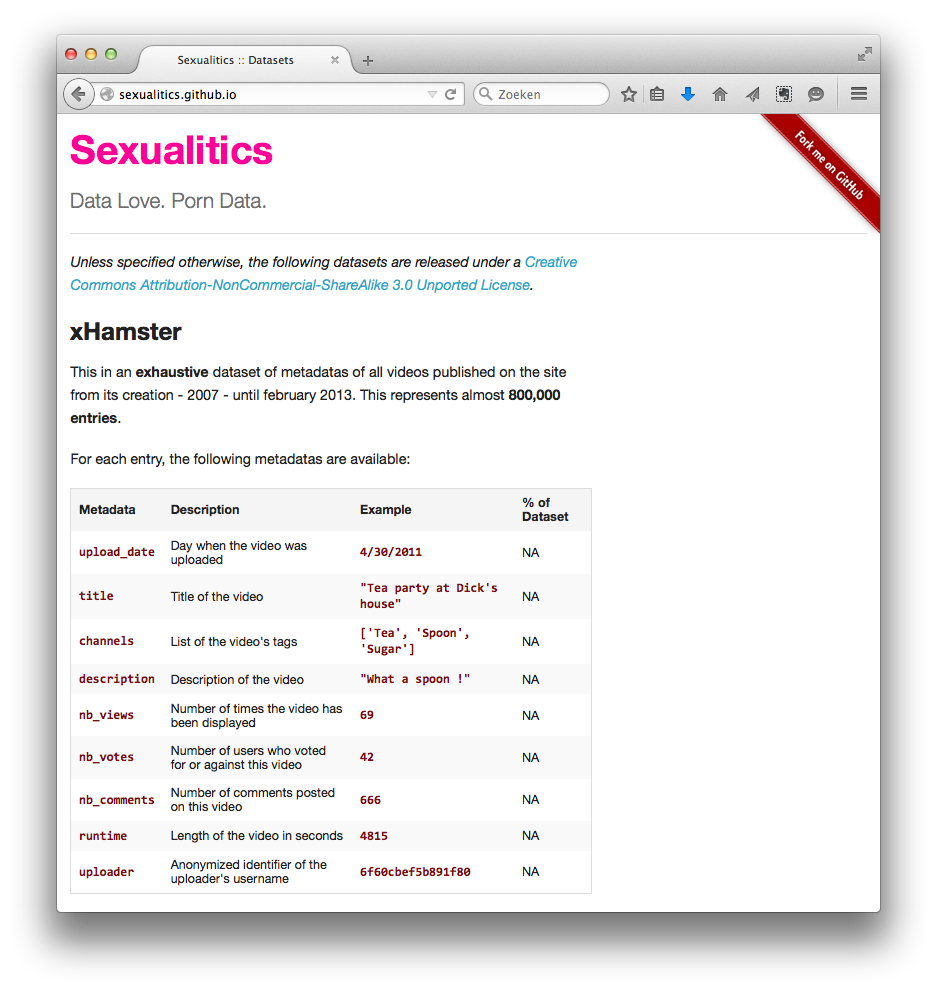
\includegraphics[width=.75\paperwidth,keepaspectratio]{../pictures/sexualitics.png}
\caption{\label{fig:sexualitics}The discription of the dataset.}
\end{figure}

We do the exercise together in class, but make sure you have downloaded the dataset before class. You can do so as follows (but, of course, replace ``damian'' with your own user name):
\begin{lstlistingbash}
cd /home/damian
mkdir pornexercise
cd pornexercise
wget pornstudies.sexualitics.org/data/xhamster.json.tar.gz
tar -xzf xhamster.json.tar.gz
\end{lstlistingbash}
The \texttt{wget} command downloads the dataset. It is compressed, so we have to uncompress it, which is done by the \texttt{tar} command (most of you probably are used to having \texttt{.zip} files for compressed or archived data, which is essentially the same; \texttt{.tar.gz} is more common among the nerdier part of the population).
Lets check if everything went right:
\begin{lstlistingbash}
ls -lh
\end{lstlistingbash}
should give you an output like this:
\begin{lstlistingoutput}
damian@damian-VirtualBox:~/pornexercise$ ls -lh
total 284M
-rw-r--r-- 1 damian damian 229M feb  8  2014 xhamster.json
-rw-rw-r-- 1 damian damian  55M feb  8  2014 xhamster.json.tar.gz
\end{lstlistingoutput}
You see that the compressed file is 55MB large, but the uncompressed one is more than four times as large. Let's delete the compressed one, we don't need it any more:
\begin{lstlistingbash}
rm xhamster.json.tar.gz
\end{lstlistingbash}

\section{The tasks}
Start with having a look at Figure~\ref{fig:sexualitics}. It is important to understand the structure of the data: Which fields are there, how are they named, and what do they contain? For example, we see that the field ``channels'' contains a \emph{list} of different tags, while ``nb\_votes'' seems to contain an \emph{integer}.
Ready to go? Let's do some work:

\begin{enumerate}
\item Print the title of each video.
\item
	\begin{enumerate} 
	 \item What are the 100 most frequently used tags?
	 \item What is the average number of tags per video?
	\end{enumerate}
\item What tags generate the most comments/votes/views?
\item What is the average length of a video description?
\item What are the most frequently used words in the descriptions?
\end{enumerate}


\chapter[Exchanging files]{Exchanging files by mounting your host system}

One of the nice things of using a Virtual Machine is that you cannot break anything on your own computer. The obvious downside is that you also cannot access files on it. Of course, you can always mail stuff to yourself or use some other workaround. 

But if you \emph{really} want to break the isolation and have access to folders on your computer, here is how it works.

The process of connecting a device (a USB stick, a harddisk, \ldots) and assigning it a name is called ``mounting''. For example, when you insert a USB stick in a Mac  or Linux computer, it might be (nowadays, usually automatically) mounted on \texttt{/media/mystick} or something similar. 

What you want to do, is mounting a directory from your ``real'' computer, the so-called host, in the file system of the VM. Select the folder you want to share in Virtual Box (see Figure~\ref{fig:mount}). Select permanent, but NOT auto-mounting (screenshot). Remember the name of the share (in my example, Desktop)

\begin{figure}[h]
\centering
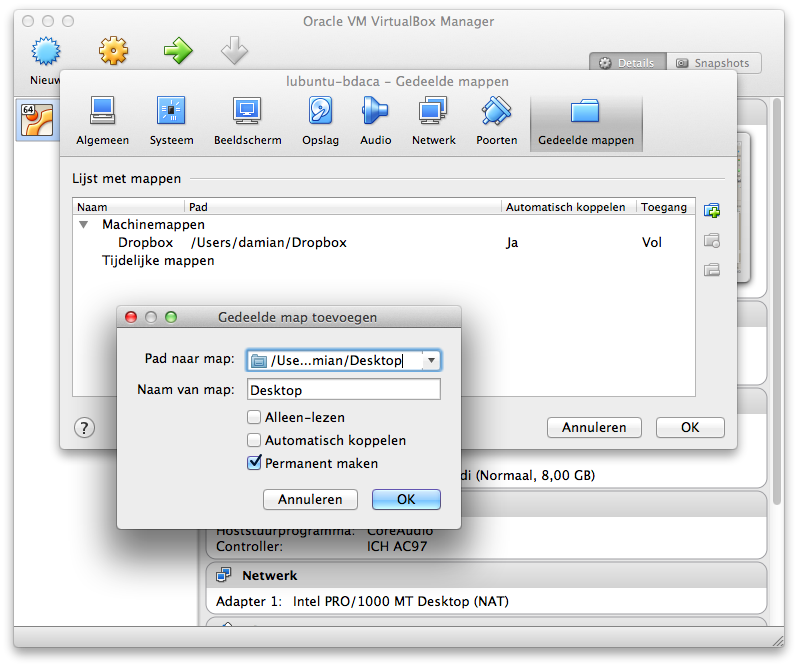
\includegraphics[width=.75\paperwidth,keepaspectratio]{../pictures/virtualbox-mount.png}
\caption{\label{fig:mount}Configuring VirtualBox to make it possible to mount folders from the host system}
\end{figure}

Within the VM, now create a folder where you want the content of your host folder to appear. For example, this could be:

mkdir /home/damian/myrealcomputer

Now, use the following line to mount the share (in my example, it is called Desktop) to that folder:

\begin{lstlistingbash}
sudo mount -t vboxsf -o uid=$UID,gid=$(id -g) Desktop /home/damian/myrealcomputer/
\end{lstlistingbash}

Voil\`a!


\chapter{Installing Python on other systems}
\label{chap:anaconda}
\textbf{Before you install Python outside of the virtual machine, read this so that you know what you are doing.} While you could just go to \url{http://python.org} and download Python for your operating system, this may or may not be a good choice. First, Python might already be installed (which you could find out by typing \texttt{python} or  \texttt{python3} in your Terminal). Second, even if it is not, if you prefer one-stop-shopping above dealing with packages, you might like Anaconda (see below).

Keep in mind that one can have multiple versions of Python on one computer, and you don't want to litter your system with a lot of different versions that you then mix up accidentally. 

In this book, we use a virtual machine with Linux as operating system. However, if you want to install Python somewhere else, chances are high that it isn't Linux. Within Linux, we used the system's package manager \texttt{apt-get} to install Python itself (and maybe some other programs). We then used \texttt{pip} to install specific Python packages. This requires you to know which packages you want (that's why we installed a bunch of them on page~\pageref{sec:installpackages}), but on the other hand, if you forgot one, it doesn't really matter because you can easily just install it later on.

All very easy, it seems, but to install some (few) packages via pip one needs specific programs like, for instance, a C compiler. You probably didn't even realize this, because on Linux, this stuff is usually present, and if not, it can be easiliy installed via \texttt{apt-get}. MacOS \emph{sometimes} has the necessary stuff installed (usually if you have installed XCode via the App Store). But on a common Windows installation, things can quickly become complicated (unless you know exactly what you are doing).

Because people do not really like dealing with all this stuff, there is an easier solution: Anaconda \url{https://www.continuum.io/downloads}.

Anaconda is a platform that includes Python together with a lot of commonly used scientific Python packages preinstalled. In addition, it has its own package manager, \texttt{conda}, which can solve some dependencies \texttt{pip} cannot resolve. 

So, if you want to use Python outside of the virtual machine that we used in this book, you might want to give Anaconda a try.

One important characteristic of anaconda is that it installs an own Python installation in your home directory. To quote from their documentation:

\begin{lstlistingoutput}
On Windows this might be a path such as C:\Users\Jane Smith\anaconda\bin\python.
On macOS this might be a path such as /Users/jsmith/anaconda/bin/python.
On Linux this might be a path such as /home/jsmith/anaconda/bin/python.
As well as anaconda, the folder in your home directory might be named anaconda2 or anaconda3.
\end{lstlistingoutput}

Because you might \emph{also} have a version of Python already installed on your system (at least on Linux and MacOS, this is generally the case), you have to make sure that you actually run the correct version: If you just type
\begin{lstlistingbash}
python
\end{lstlistingbash}
in your Terminal, then you probably will \emph{not} start the anaconda version -- and thus be unable to use the packages installed with anaconda. You would have to explicitly refer to the location where anaconda is installed.

\end{appendices}

\backmatter



\bibliographystyle{apacite}
\bibliography{../bdaca}

\end{document}